% ================================================
% =                 METHODOLOGY                  =
% ================================================ 

This section details the experiments and implementations made to address the problems described in section \ref{Introduction}. On the first hand, the experimental design is introduced, tackling the model and dataset selection, how data augmentations are performed and the training and validation processes. Afterward, the implementation of the occupancy and occlusion masks preannotation pipeline is presented. Finally, the evaluation strategy of the pipeline is discussed to measure the quality of the resulting semantic masks and the monocular 3D detections for estimating the object's dimensions.

Thus, this project can be divided into three main blocks: \aclink{BEV} semantic segmentation experimentation, design and implementation of the preannotation pipeline and a thrid block of how the system is evaluated.

\subsection{Segmentation experiment design: BEV2Seg\_2}
\label{bev2seg_2}

To address the hypotesis that "A semantic segmentation model trained with BEV images better segments planar elements" the process represented in Figure \ref{fig:beg2seg_2_flow} has been designed. It follows two main approaches: first, performing image segmentation on regular RGB images and then reprojecting them to \aclink{BEV}; second, applying \aclink{IPM} to the original images and then segmenting them with the model.

\begin{figure}[h!]
    \centering
    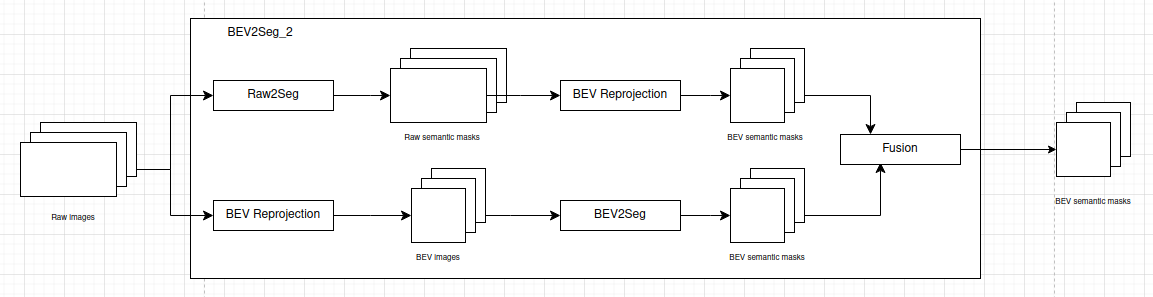
\includegraphics[width=\linewidth]{./images/metodology/bev2seg_2_flow.png}
    \caption{bev2seg\_2 flow diagram.}
    \label{fig:beg2seg_2_flow}
\end{figure}

Considering this flowchart, three main questions arises: (1) which segmentation model to use, (2) which dataset to train the models with, and (3) how to compare the train models and select the optimal output of the pipeline. 

\subsubsection{Segformer}
There are multiple techniques and strategies for tackling semantic segmentation in both regular and \aclink{BEV} images \ref{sota}.  

Several models could be chosen to address the proposed hypothesis. The current state of the art includes both \aclink{CNN} and \aclink{ViT}-based models that achieve competitive results. As shown in Figure \ref{tab:model_comparison}, there is no significant difference in accuracy and inference speed among the top-performing models. Moreover, many of these models have already been applied in the context of \aclink{ADS}. In this work, Segformer \cite{segformer} has been selected as the semantic segmentation model due to its balance between performance and efficiency. Additionally, it is integrated into the Huggingface \cite{huggingface} ecosystem, which provides an optimized, parallelized implementation, facilitating distributed training.  

\begin{table}[h]
    \centering
    \resizebox{\linewidth}{!}{%
    \begin{tabular}{l l c c c}
        \toprule
        \textbf{Model Name} & \textbf{Encoder} & \textbf{Params (M)} $\downarrow$ & \textbf{FPS} $\uparrow$ & \textbf{Cityscapes test mIoU ($\%$)} $\uparrow$ \\
        \midrule
        DDRNet-39       & -             & 32.3      & -         & 80.4 \\
        PIDNet-L        & -             & 36.9      & -         & 80.6 \\      
        DeeplabV3+      & ResNet-101    & 62.7      & 1.2       & 80.9 \\
        SETR            & ViT-Large     & 318.3     & 0.5       & 82.2 \\
        Segformer       & MiT-B4        & 64.1      & 3.0       & 83.8 \\
        \bottomrule
    \end{tabular}%
    }
    \caption{Comparison of different models. Results are obtained from \cite{DDRNet} \cite{PIDNet} \cite{segformer}.  }
    \label{tab:model_comparison}
\end{table}


The Segformer model consists on an hierarchical Transformer  encoder, which extract coarse and fine features, and a lightweight \aclink{MLP} decoder to directly fuse these multiscale features and predict the segmentation mask (Figure \ref{fig:segformer_architecture}). Segformer comes with a series of Mix Transformer encoders (MiT) that share the same architecture but have different sizes: from MiT-B0 as the lightweigtest encoder for realtime inference, to MiT-B5 for best performance.

\begin{figure}[h!]
    \centering
    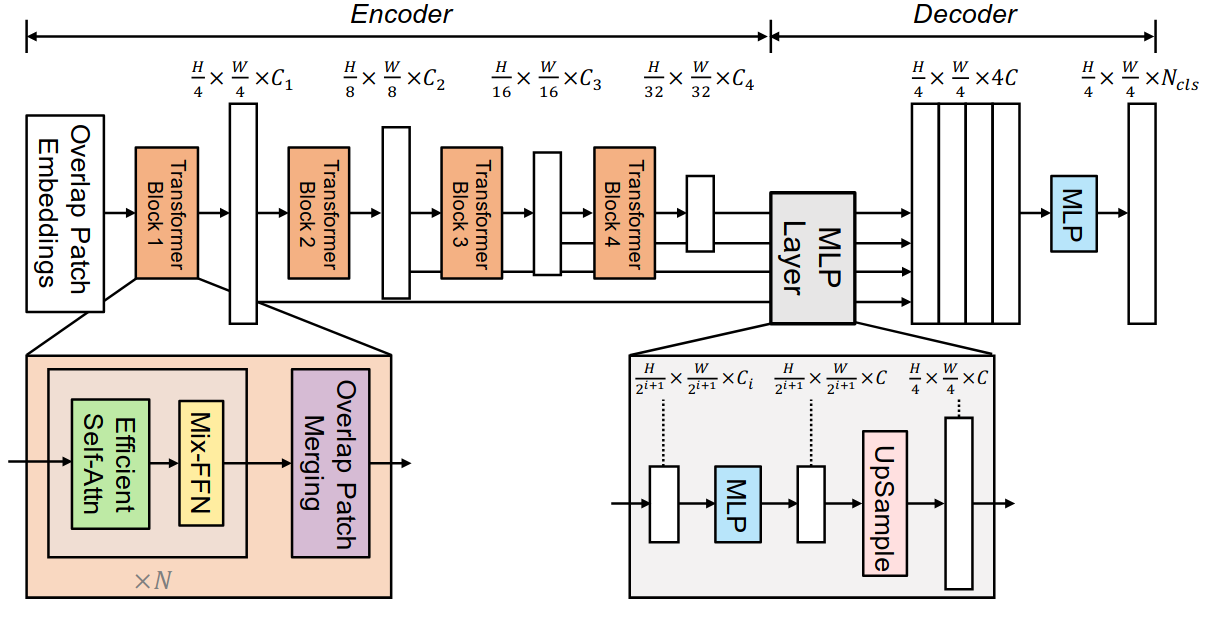
\includegraphics[width=\linewidth]{images/metodology/segformer_architecture.png}
    \caption{Segformer architecture}
    \label{fig:segformer_architecture}
\end{figure}

The training strategy involves using pretrained encoders from ImageNet-1K, attaching an untrained segmentation head decoder, and fine-tuning the entire model for semantic segmentation of vehicular scenes. Since the objective is to train the models directly on \aclink{BEV} images, which differ significantly from standard perspective images, the encoder layers will remain trainable rather than being frozen.


\subsubsection{BEVDataset}
In order to train the model on the segmentation task, a valid dataset must be selected. There are several semantic segmentation datasets for the \aclink{ADS} context such as Cityscapes \cite{Cityscapes}, that defines $30$ semantic classes and provides $5.000$ frames with pixel-level high-quality annotations and $20.000$ weakly annotated images; KITTI \cite{KITTI}, which provices $400$ annotated images with a $0.5$ split for training and validation following the Cityscapes annotation format; ApolloScape \cite{ApolloScape}, that provides $146.997$ frames with corresponding pixel-level annonations and pose information for $25$ labels; or NuImages, a subset of NuScenes \cite{nuscenes}, that contains annotated images on $26$ different labels. For all of them, the ego pose and camera parameters metadata are provided. 

There are other benchmarks \cite{WildDash} \cite{CamVid} but in orther to train the models a rich dataset is needed. Despite Cityscapes and ApolloScape being good options for this task, NuImages has been selected as it is one of the most used datasets for \aclink{ADS} tasks, it provides very accurate ego poses and camera parameters, it has 3D annotations and it has a very good documentation.

NuImages contains around $93.000$ samples with aproximately $80\%$ reserved for the training set and $20\%$ for validation. Additionally, NuImages includes a private test set reserved for benchmark evaluations, whose annotations are not publicly available.

To train the models in the pipeline, a parser has been developed to convert NuImages into a sub-dataset named BEVDataset. This dataset has all front-camera images with NuImages annotations. Since the test annotations in NuImages are private, the validation set has been further splitted to ensure fair comparisons between models from different pipelines.

The conversion process is performed using a custom parser named "OLDatasets", which transforms NuImages samples into the structured ASAM OpenLABEL \footnote{\url{https://www.asam.net/standards/detail/openlabel/}} format, where metadata for each frame is stored. In the case of BEVDataset, images are reprojected into the \aclink{BEV} domain using the \aclink{VCD} library \cite{VCD}. This library provides tools to handle OpenLABEL annotations and manage both 2D and 3D data efficiently.

The "OLDatasets" parser extracts the camera parameters for each sample and computes a \aclink{LUT} to apply \aclink{IPM} reprojection. Using this data, semantic pixel masks are generated and reprojected along with the original images into the \aclink{BEV} space. Since this reprojection involves image warping, the interpolation method must be carefully chosen:
\begin{itemize}
    \item Linear interpolation is applied to images.
    \item Nearest neighbor interpolation is used for semantic masks to preserve pixel class integrity. 
\end{itemize}

The virtual \aclink{BEV} camera parameters are fixed: \aclink{BEV} reprojection is generated using a regular grid with a cell spacing of 1 meter, covering a total distance of 30 meters in front of the camera and 1 meter behind it. The resulting images have a resolution of $1024 \times 1024$ pixels.

Finally, BEVDataset contains a total of $16.427$ images, distributed as shown in Figure \ref{fig:bev_dataset}.

\begin{figure}[h!]
    \centering
    \includegraphics[width=\linewidth]{images/metodology/BEVDataset.png}
    \caption{BEVDataset structure and mini set samples}
    \label{fig:bev_dataset}
\end{figure}


\subsubsection{Data augmentations}
\label{data_augmentations}
Data augmentations are commonly used in deep learning models to mitigate overfitting during training and improve model generalization. There exists multiple types of data augmentation on the image domain: from pixel-based transformations, such as color space modifications, histogram equalization or filtering operations; to geometric transformations, including translations, rotations, shearings and homographies. These techniques have been widely applied in computer vision tasks and have shown to enhance model performance. However, performing data augmentation in \aclink{BEV} is not an easy task, as \aclink{IPM} images are already homographies of camera images, resulting in inherent distorsions.

Filtering operations can be applied to both standard and \aclink{BEV} images but geometric transformations were selected as the primary data augmentation method for camera domain images following the strategies employed in training the SegFormer model \cite{segformer}. Accordingly, random resizing, random cropping, and horizontal flipping were chosen as augmentation operations for perspective images.

Regarding \aclink{BEV} data augmentations, some multi-view methods implement strategies such as random flipping and random scaling, while others operate in the frequency domain \cite{HSDA}. However, these approaches apply augmentations to perspective images before the BEV transformation. Performing random cropping on a \aclink{BEV} image may lead to significant information loss, as large portions of the image may consist of unlabeled background data, potentially resulting in crops with insufficient information for effective training (Figure \ref{fig:bev_cropping}). 

\begin{figure}[h]
    \centering
    % Row labels
    \setlength{\tabcolsep}{1pt}  % Reduce column padding
    \renewcommand{\arraystretch}{0.5}
    \begin{tabular}{c c c c c c c c}

        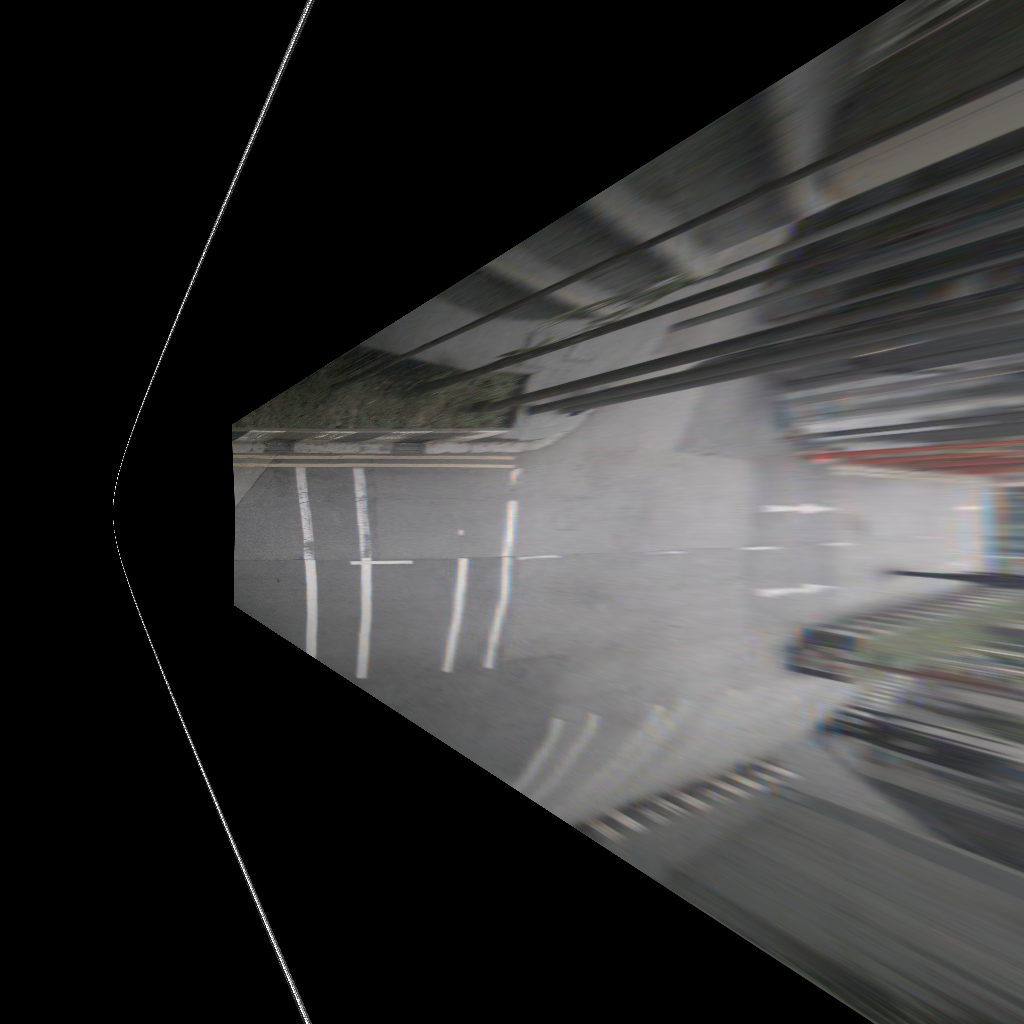
\includegraphics[width=0.12\textwidth]{images/metodology/mini/mini_0_bev.png} & 
        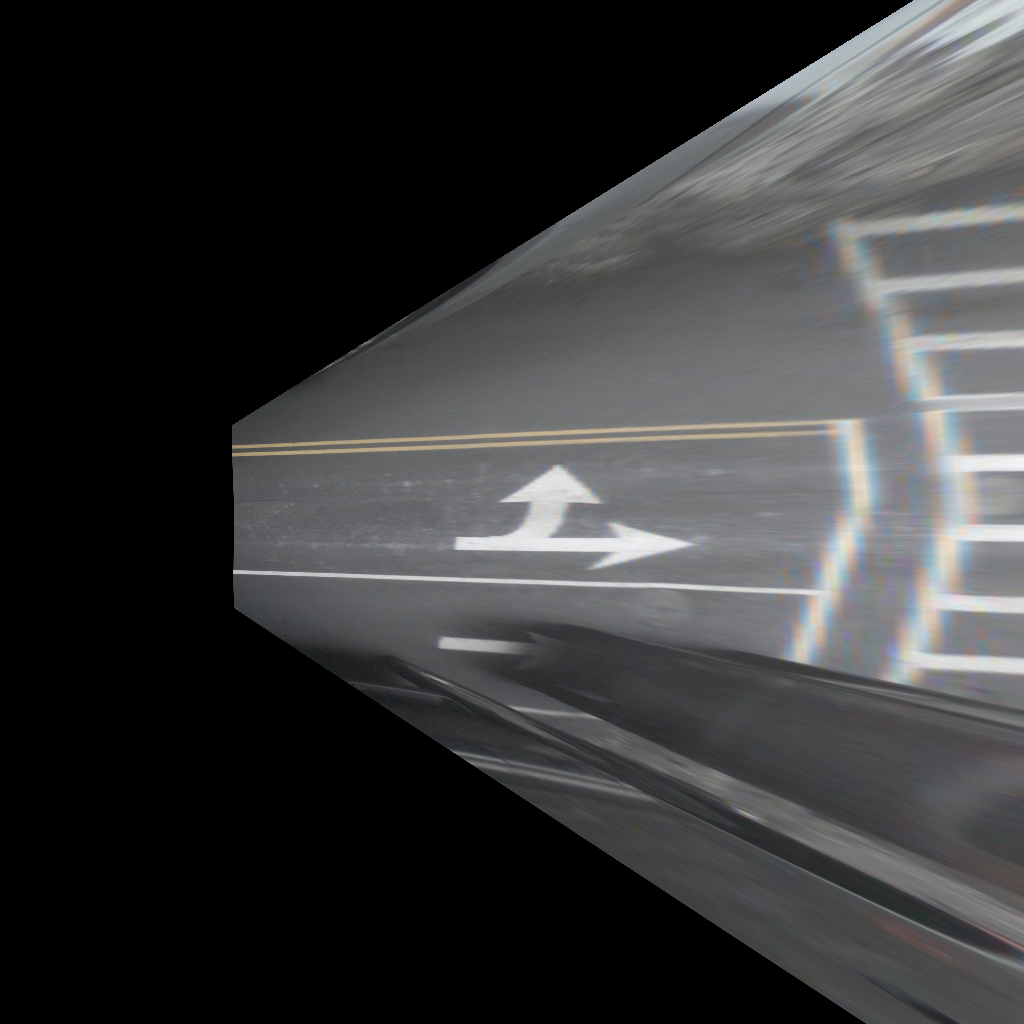
\includegraphics[width=0.12\textwidth]{images/metodology/mini/mini_1_bev.png} & 
        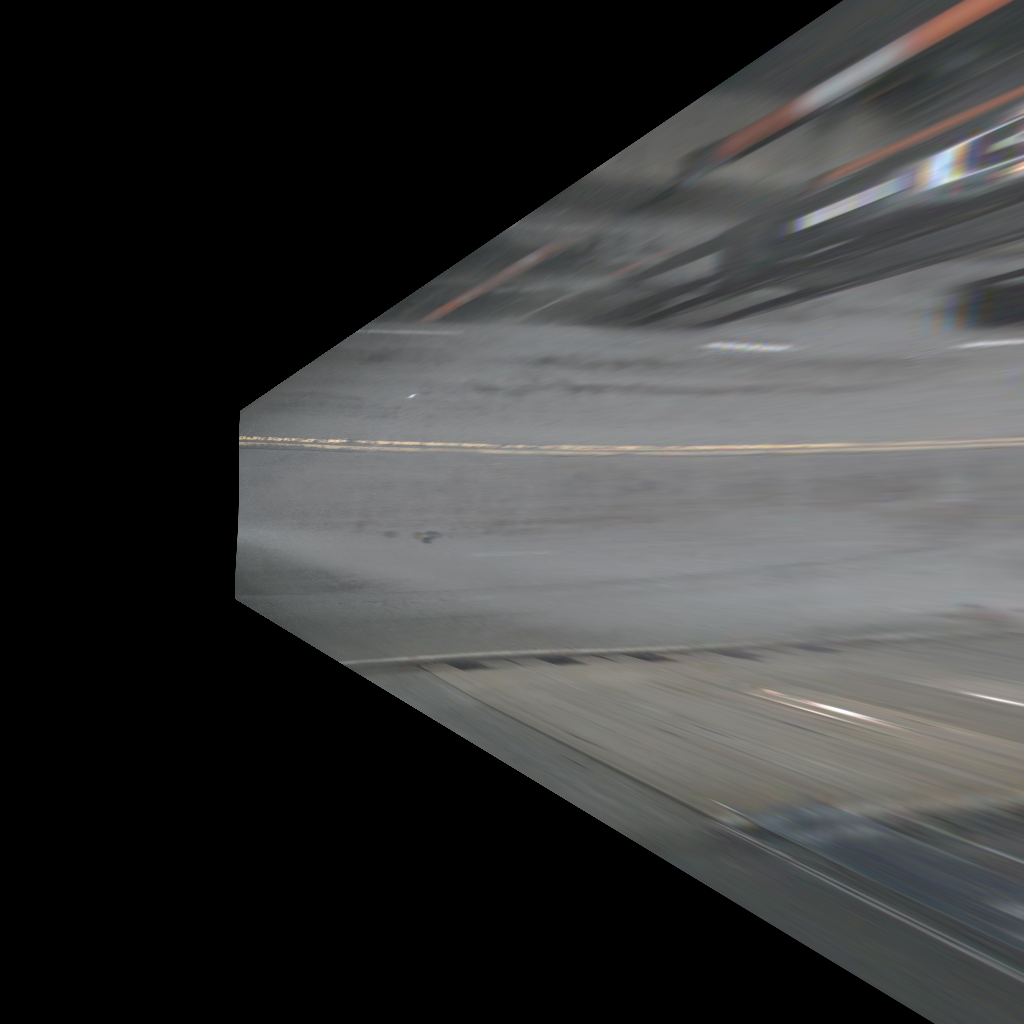
\includegraphics[width=0.12\textwidth]{images/metodology/mini/mini_2_bev.png} &
        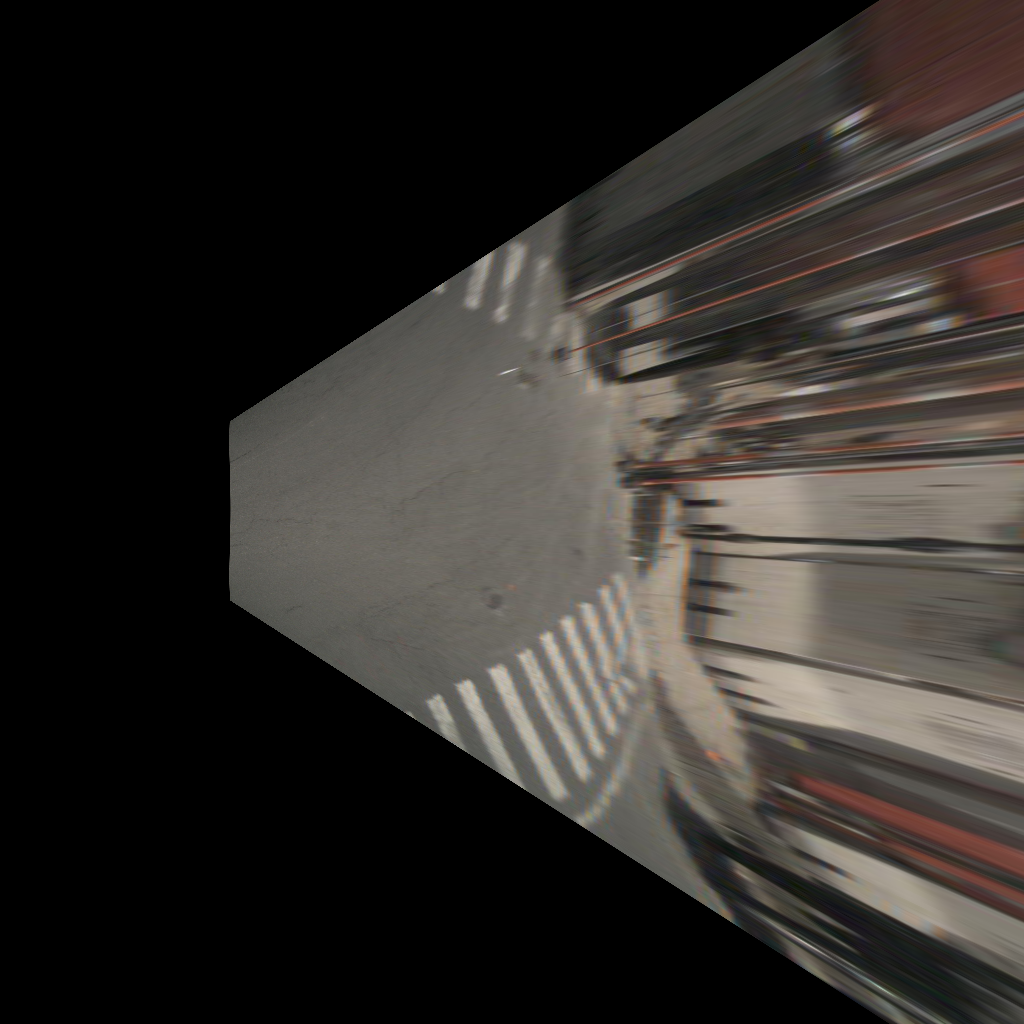
\includegraphics[width=0.12\textwidth]{images/metodology/mini/mini_3_bev.png} & 
        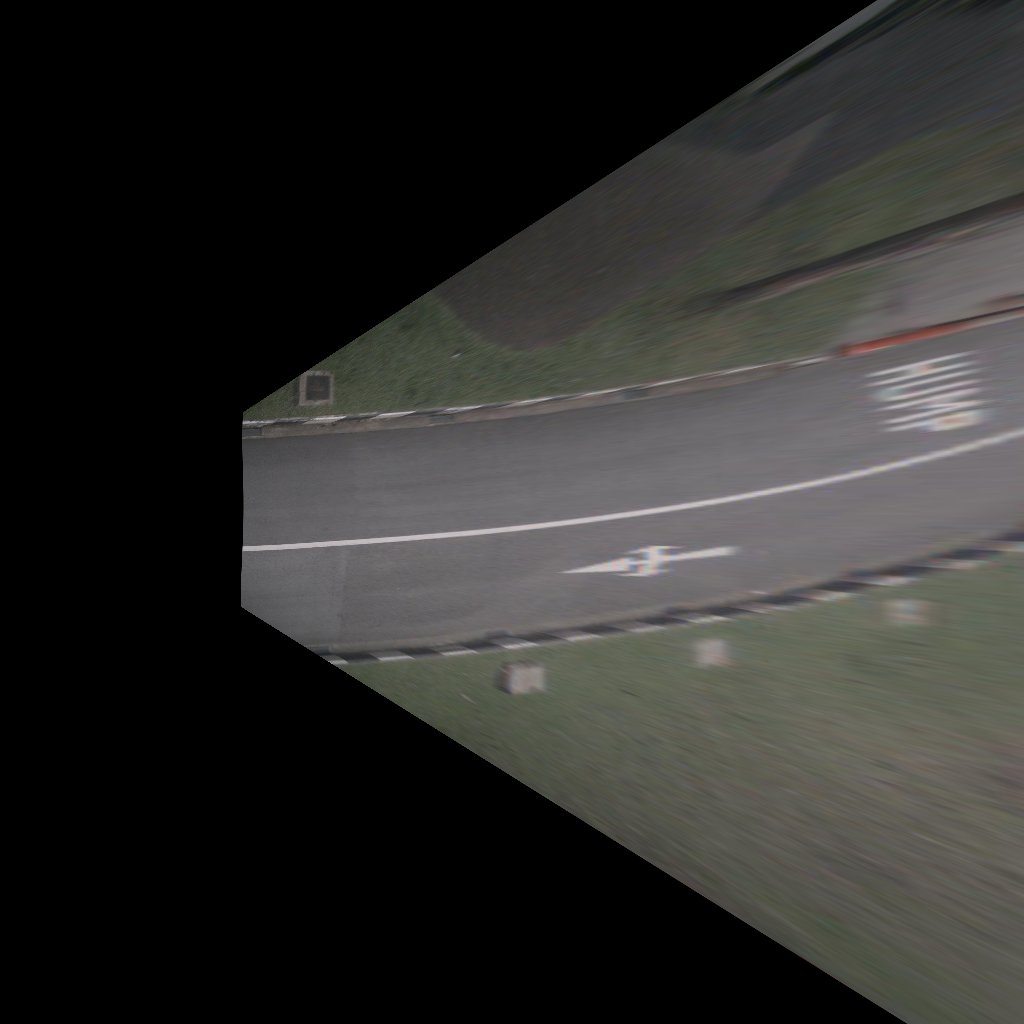
\includegraphics[width=0.12\textwidth]{images/metodology/mini/mini_4_bev.png} & 
        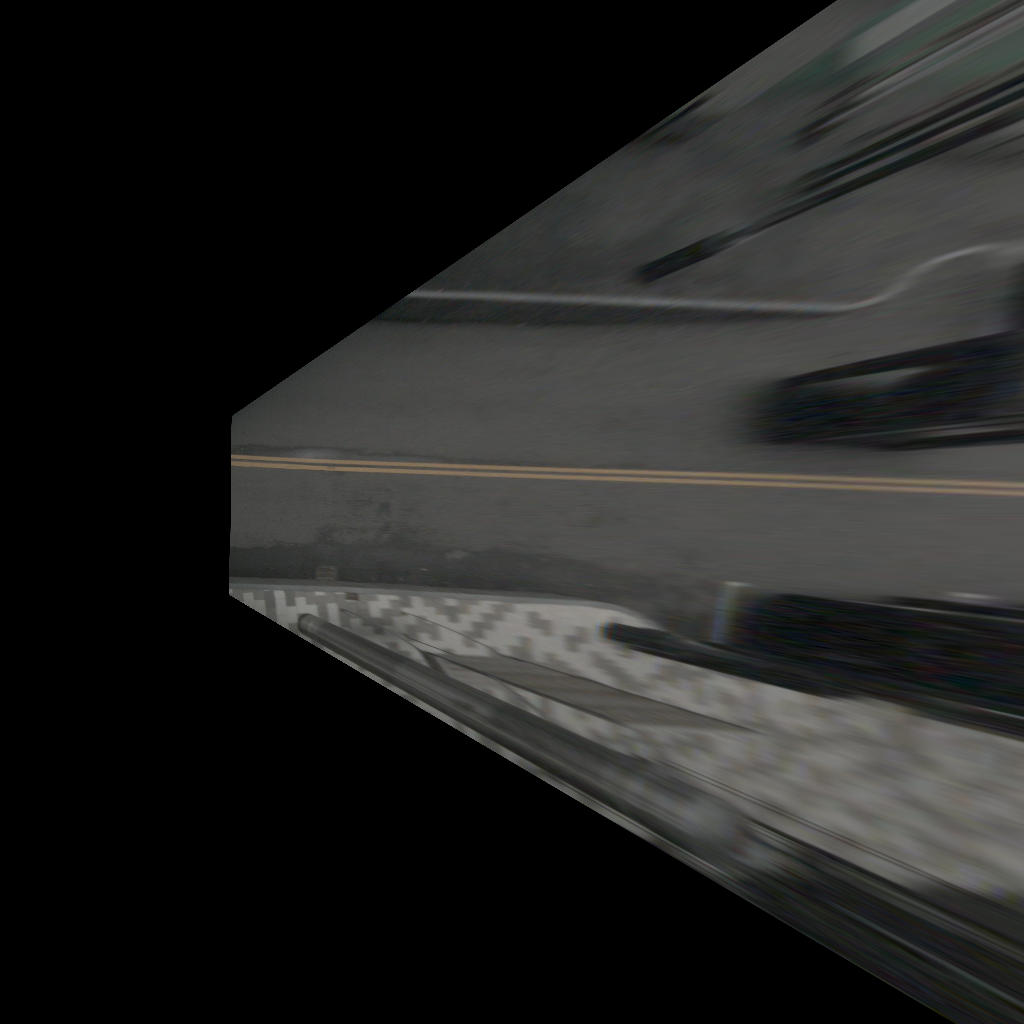
\includegraphics[width=0.12\textwidth]{images/metodology/mini/mini_5_bev.png} &
        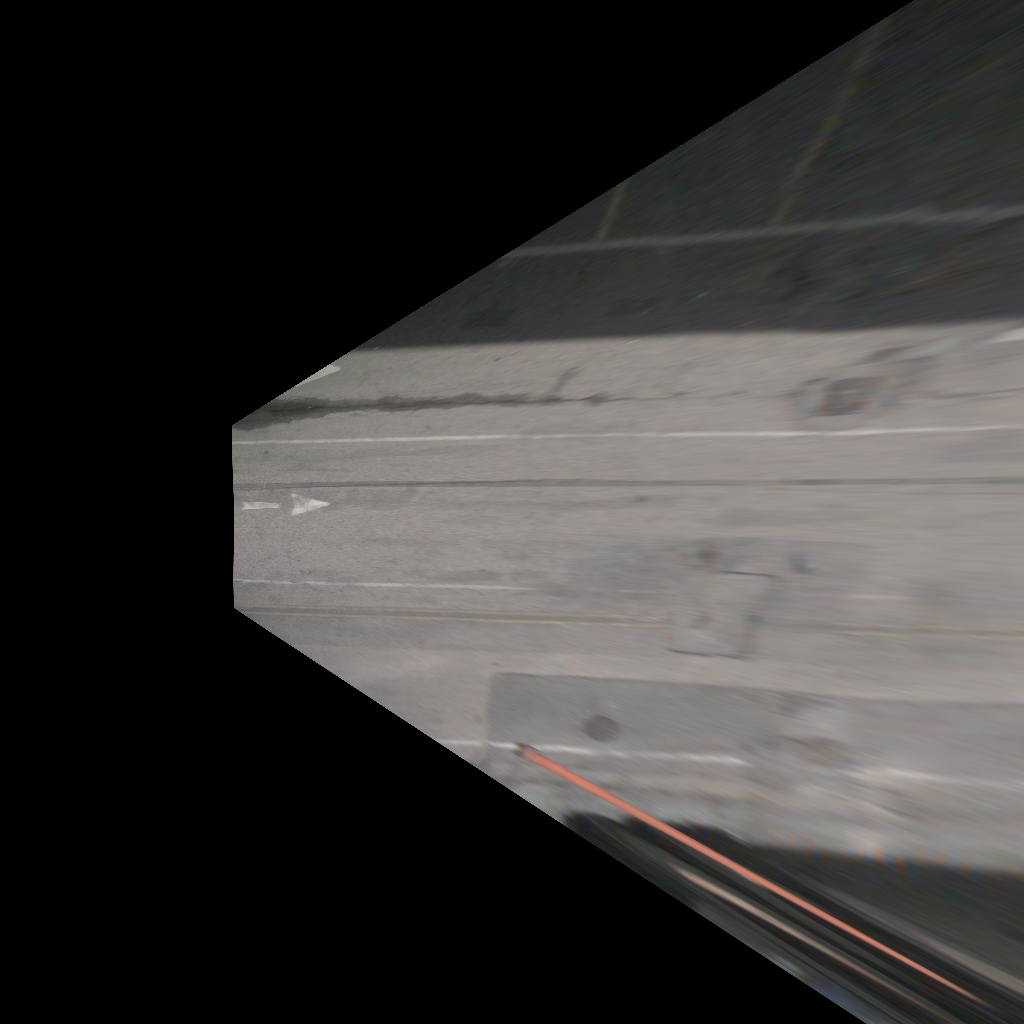
\includegraphics[width=0.12\textwidth]{images/metodology/mini/mini_6_bev.png} &
        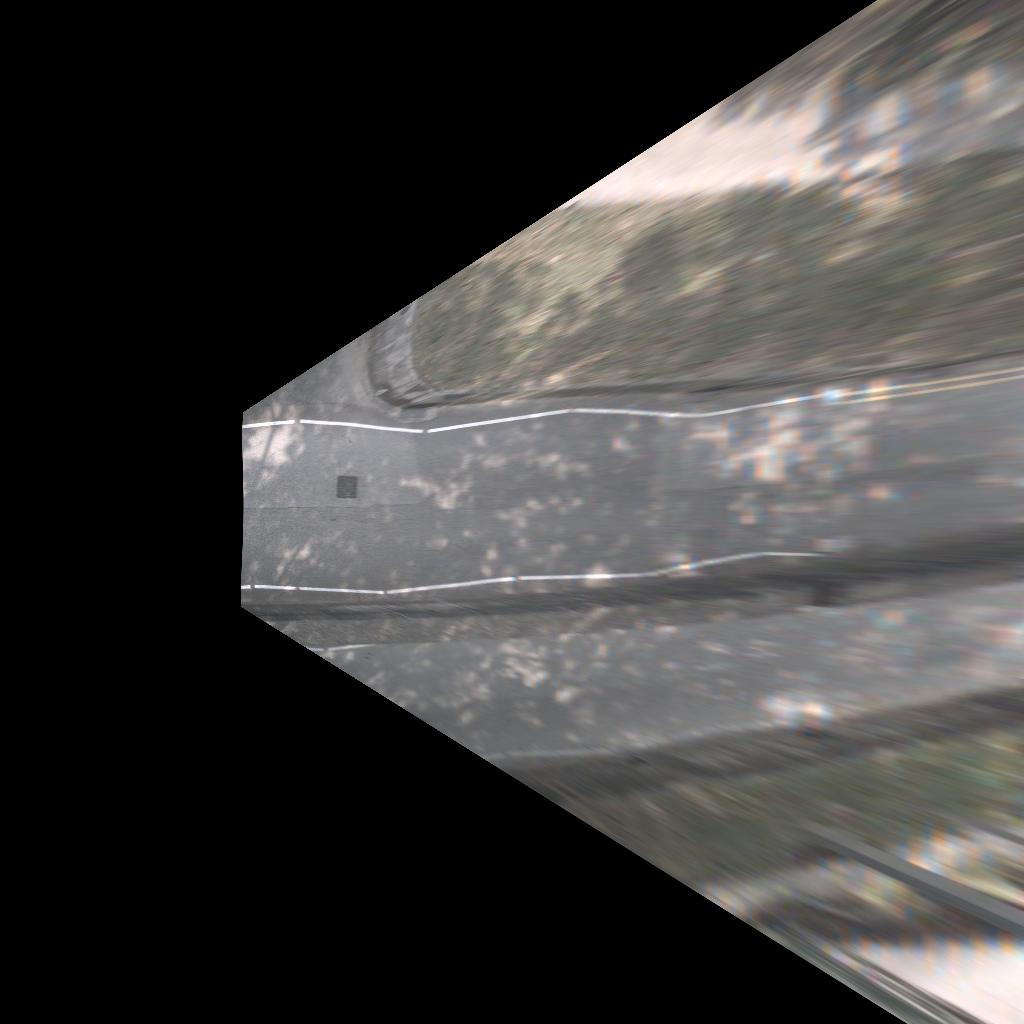
\includegraphics[width=0.12\textwidth]{images/metodology/mini/mini_7_bev.png} \\ 
        
        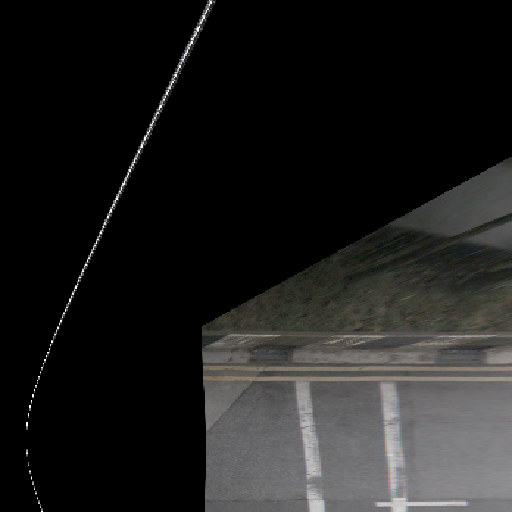
\includegraphics[width=0.12\textwidth]{images/metodology/data_augmentations/bev_crop_image_0_9.png} & 
        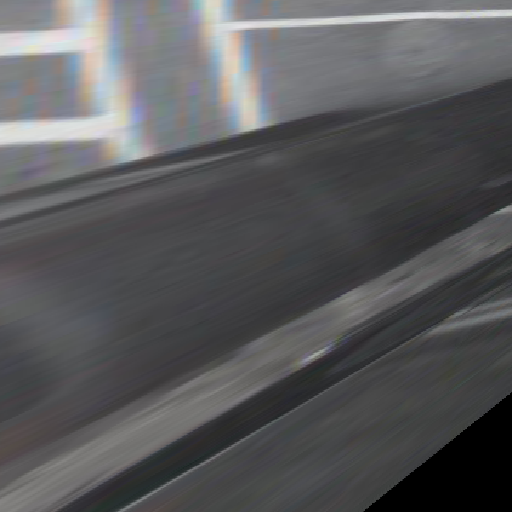
\includegraphics[width=0.12\textwidth]{images/metodology/data_augmentations/bev_crop_image_1_2.png} & 
        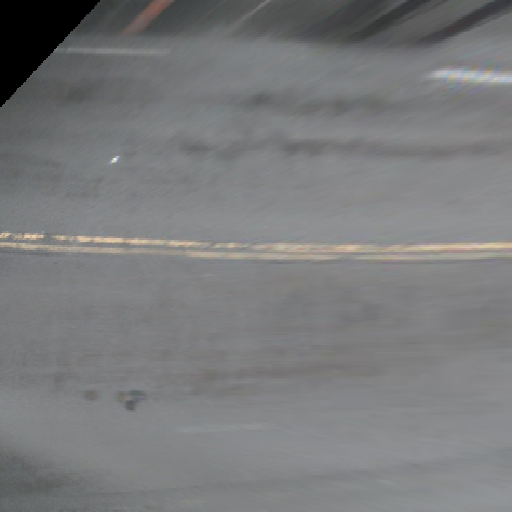
\includegraphics[width=0.12\textwidth]{images/metodology/data_augmentations/bev_crop_image_2_5.png} &
        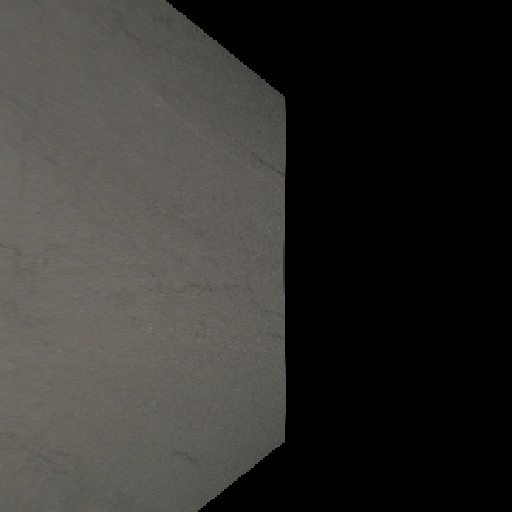
\includegraphics[width=0.12\textwidth]{images/metodology/data_augmentations/bev_crop_image_3_5.png} & 
        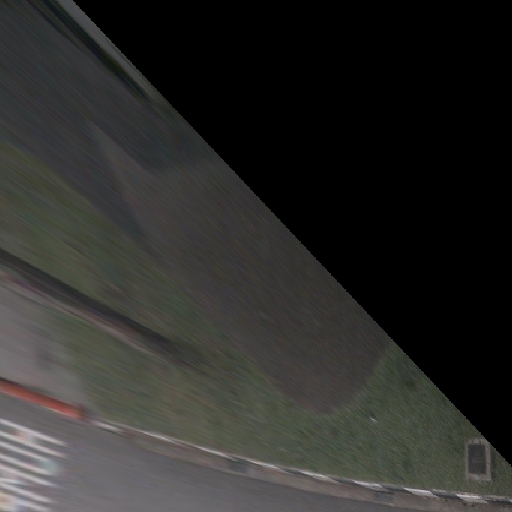
\includegraphics[width=0.12\textwidth]{images/metodology/data_augmentations/bev_crop_image_4_3.png} & 
        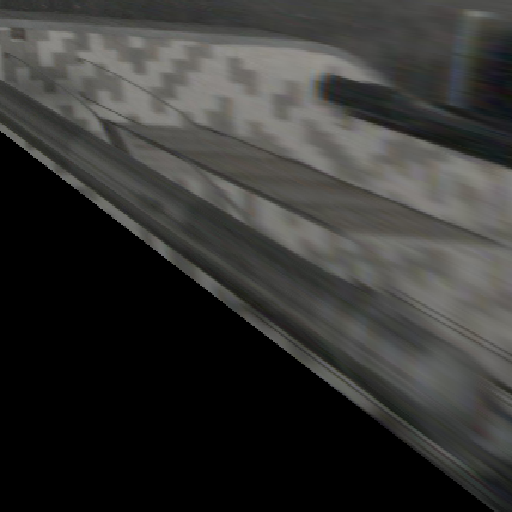
\includegraphics[width=0.12\textwidth]{images/metodology/data_augmentations/bev_crop_image_5_2.png} &
        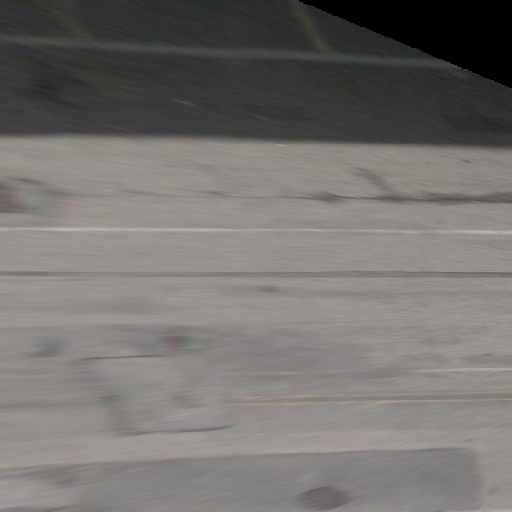
\includegraphics[width=0.12\textwidth]{images/metodology/data_augmentations/bev_crop_image_6_1.png} &
        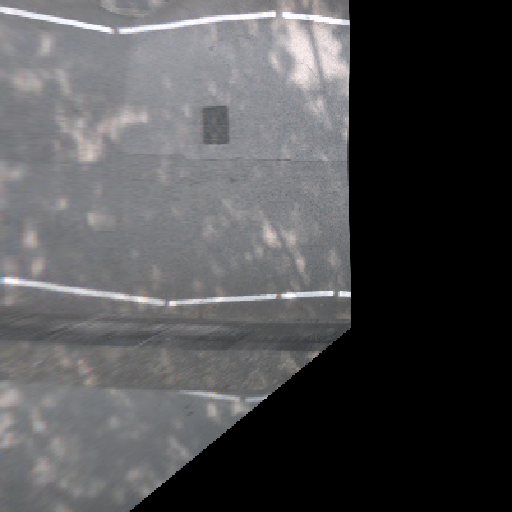
\includegraphics[width=0.12\textwidth]{images/metodology/data_augmentations/bev_crop_image_7_2.png} \\ 

        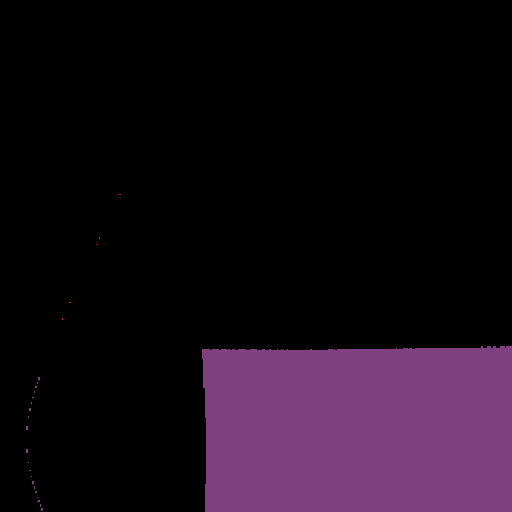
\includegraphics[width=0.12\textwidth]{images/metodology/data_augmentations/bev_crop_mask_0_9.png} & 
        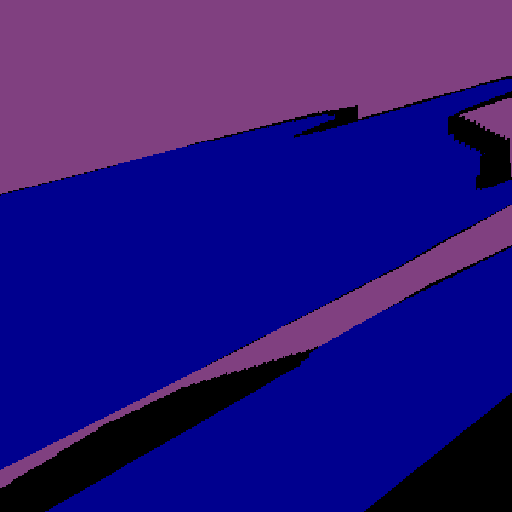
\includegraphics[width=0.12\textwidth]{images/metodology/data_augmentations/bev_crop_mask_1_2.png} & 
        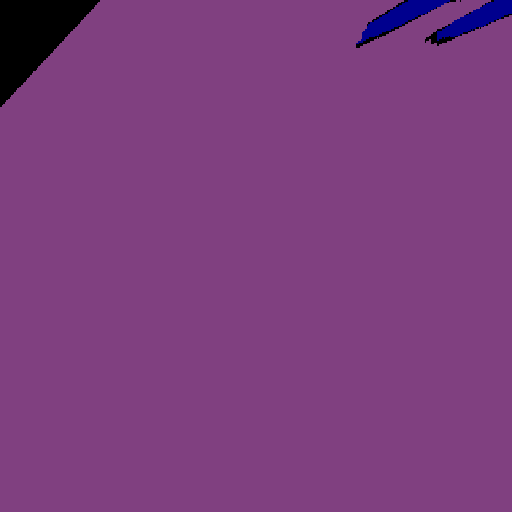
\includegraphics[width=0.12\textwidth]{images/metodology/data_augmentations/bev_crop_mask_2_5.png} &
        
\includegraphics[width=0.12\textwidth]{images/metodology/data_augmentations/bev_crop_mask_3_5.png} & 
        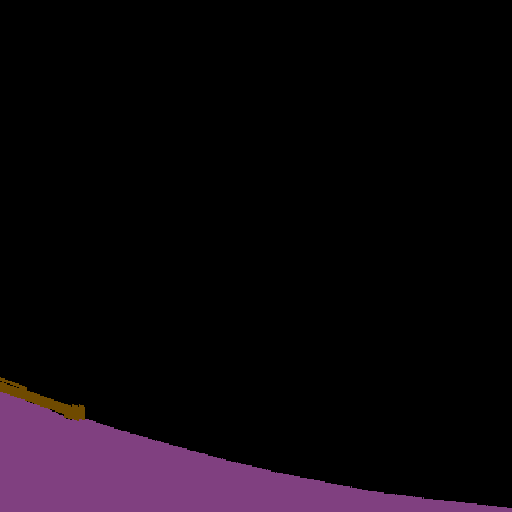
\includegraphics[width=0.12\textwidth]{images/metodology/data_augmentations/bev_crop_mask_4_3.png} & 
        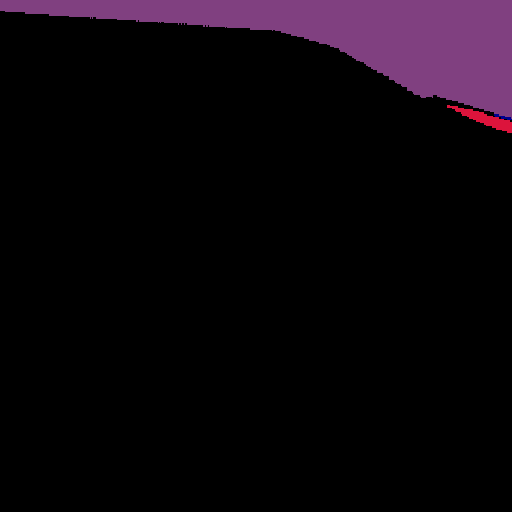
\includegraphics[width=0.12\textwidth]{images/metodology/data_augmentations/bev_crop_mask_5_2.png} &
        
\includegraphics[width=0.12\textwidth]{images/metodology/data_augmentations/bev_crop_mask_6_1.png} &
        
\includegraphics[width=0.12\textwidth]{images/metodology/data_augmentations/bev_crop_mask_7_2.png} \\

    \end{tabular}
    
    \caption{Random cropping and horizontal flipping on BEV images. Original BEV images on first row; random flipped and cropped images on second row and corresponding semantic masks on last row.}
    \label{fig:bev_cropping}
\end{figure}

In this context, a different approach was also considered: applying geometric transformations by modifying the camera's extrinsic parameters before reprojecting to \aclink{BEV} space. The objective is to introduce random transformations along one of the camera’s rotation axes, generating diverse \aclink{BEV} reprojections with varying degrees of distortion. This technique may enable the model to adapt to different extrinsic camera configurations, improving its robustness to variations in camera placement and orientation (Figure \ref{fig:bev_data_aug}).

\begin{figure}[h]
    \centering
    % Row labels
    \setlength{\tabcolsep}{1pt}  % Reduce column padding
    \renewcommand{\arraystretch}{0.5}
    \begin{tabular}{c c c c c c}
        & $-0.25$ rad & $-0.125$ rad & $0.0$ rad & $0.125$ rad & $0.25$ rad \\ 
        
        \rotatebox{90}{\textbf{Yaw}} & 
        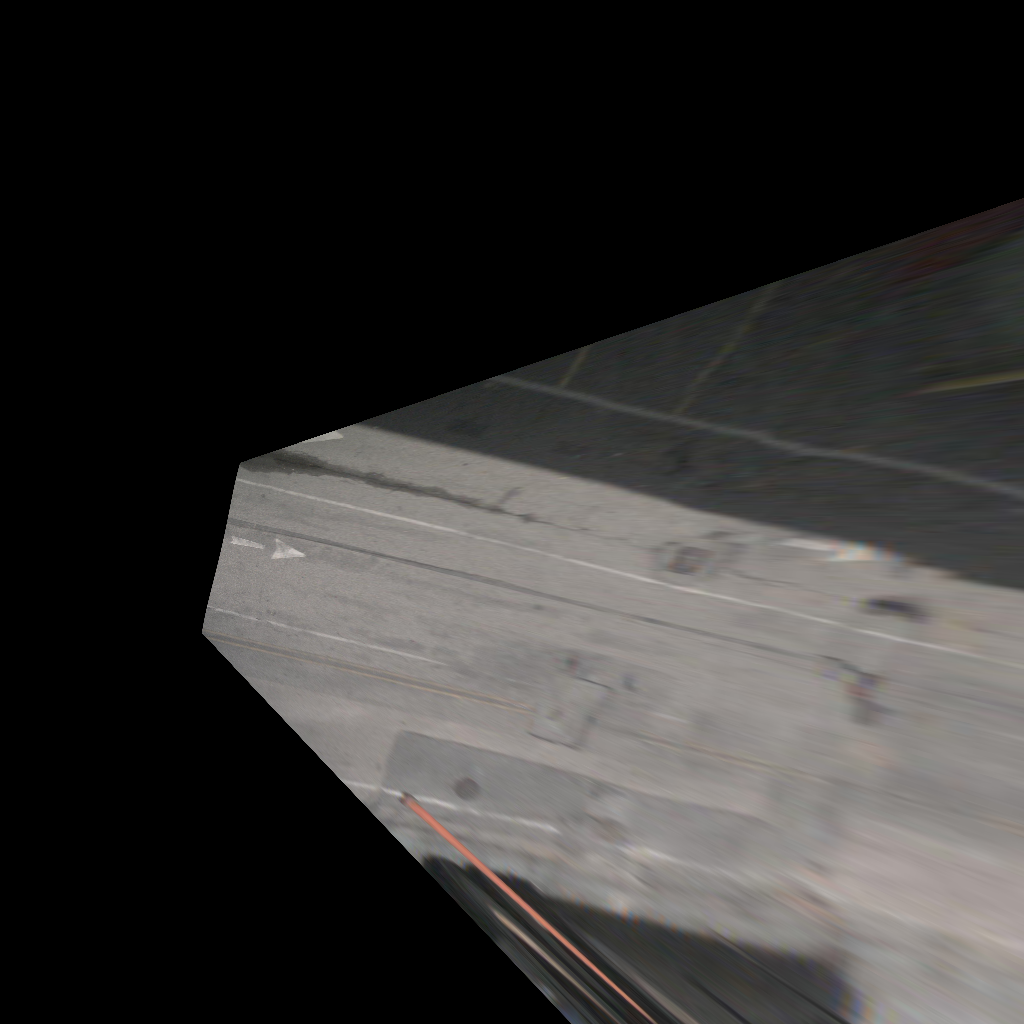
\includegraphics[width=0.15\textwidth]{images/metodology/data_augmentations/rx_-0.25_0.png} & 
        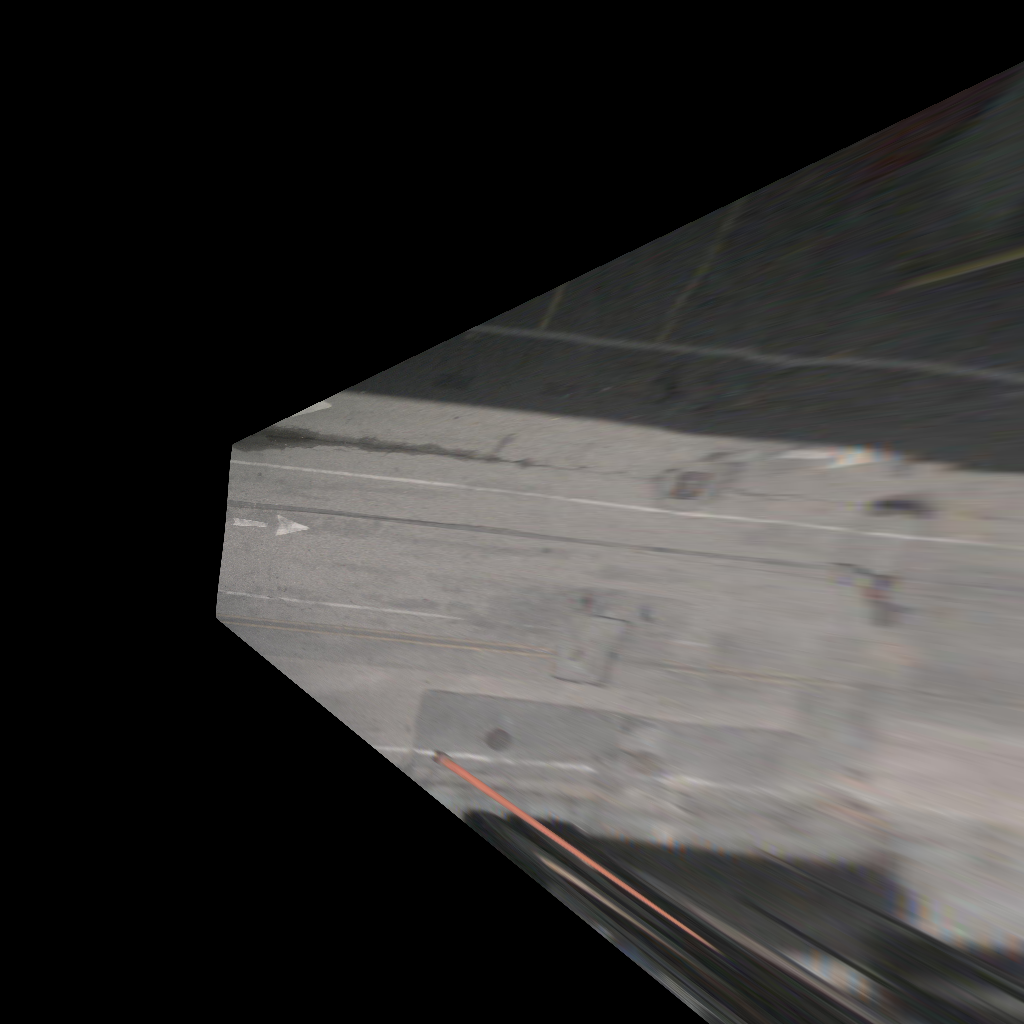
\includegraphics[width=0.15\textwidth]{images/metodology/data_augmentations/rx_-0.125_1.png} & 
        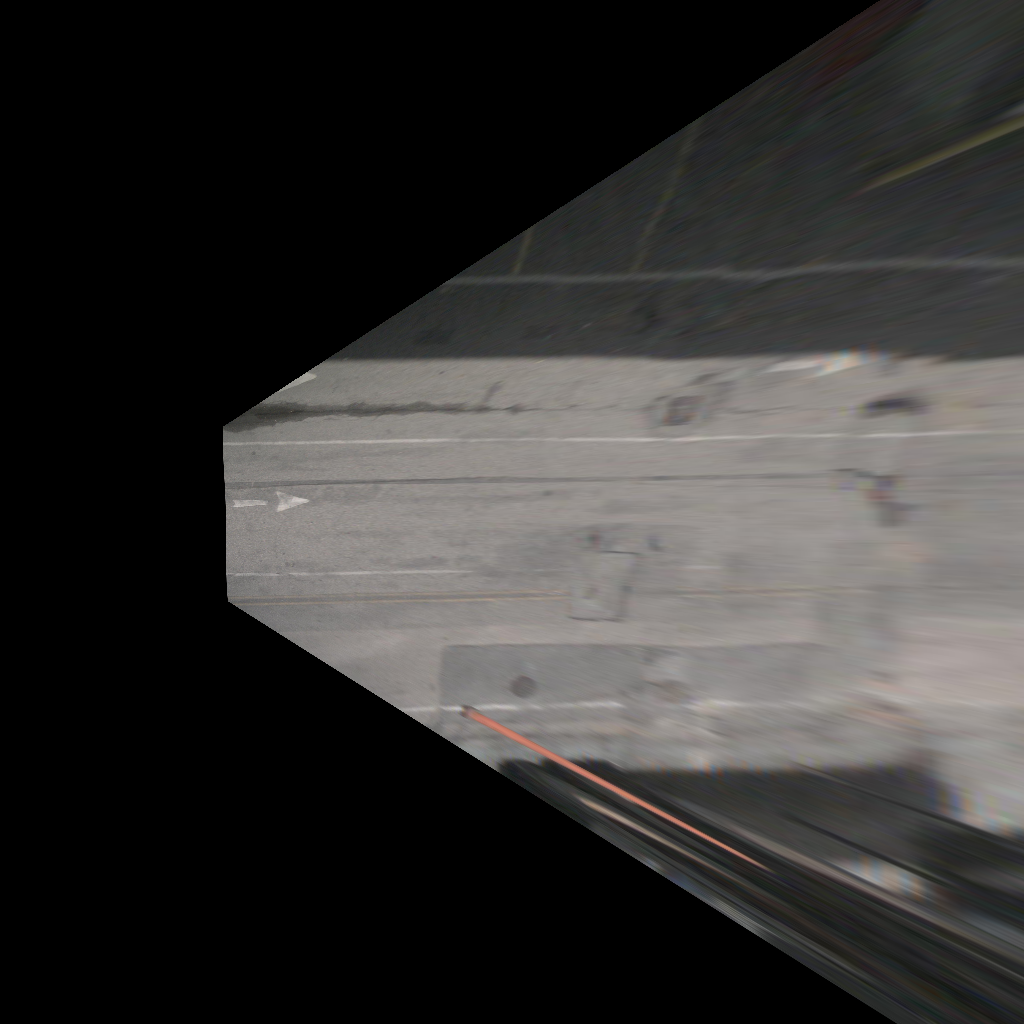
\includegraphics[width=0.15\textwidth]{images/metodology/data_augmentations/rx_0.0_2.png} & 
        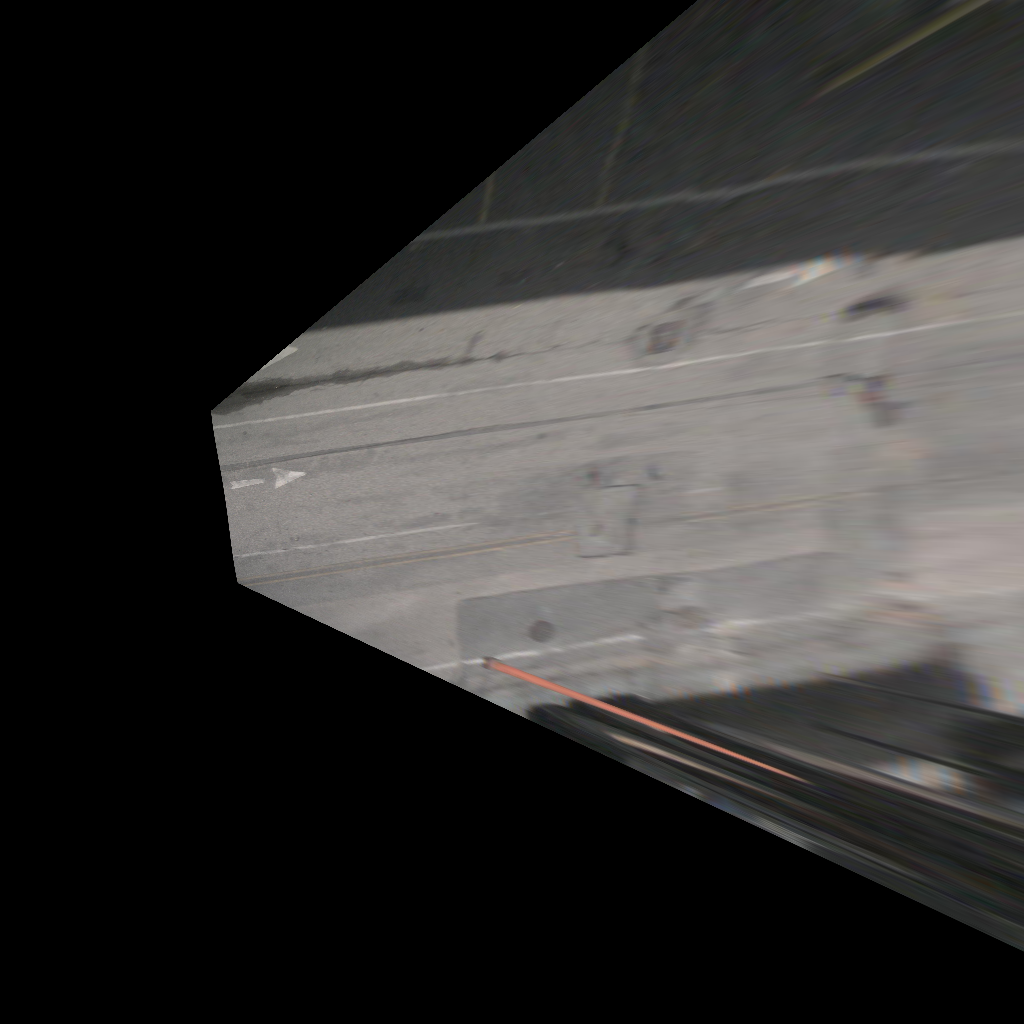
\includegraphics[width=0.15\textwidth]{images/metodology/data_augmentations/rx_0.125_3.png} & 
        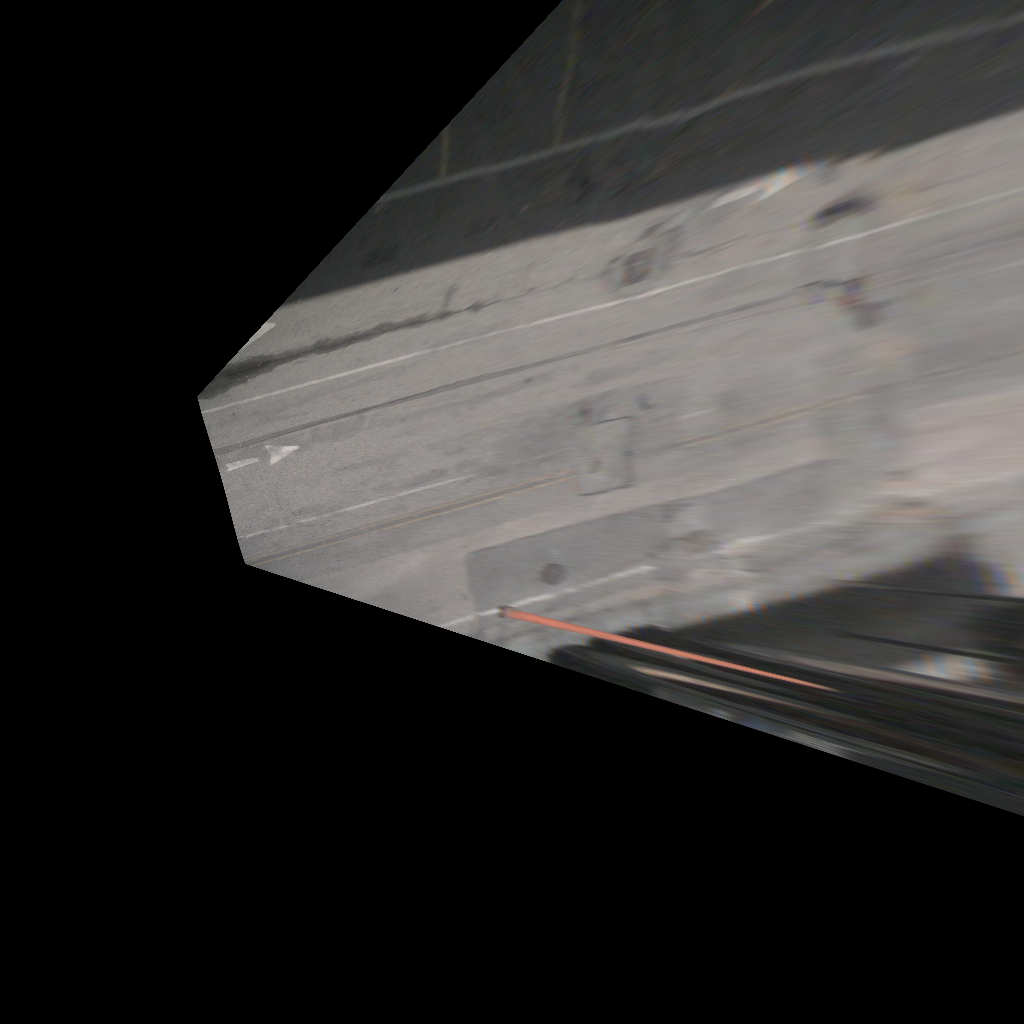
\includegraphics[width=0.15\textwidth]{images/metodology/data_augmentations/rx_0.25_4.png} \\ 
        
        \rotatebox{90}{\textbf{Pitch}} & 
        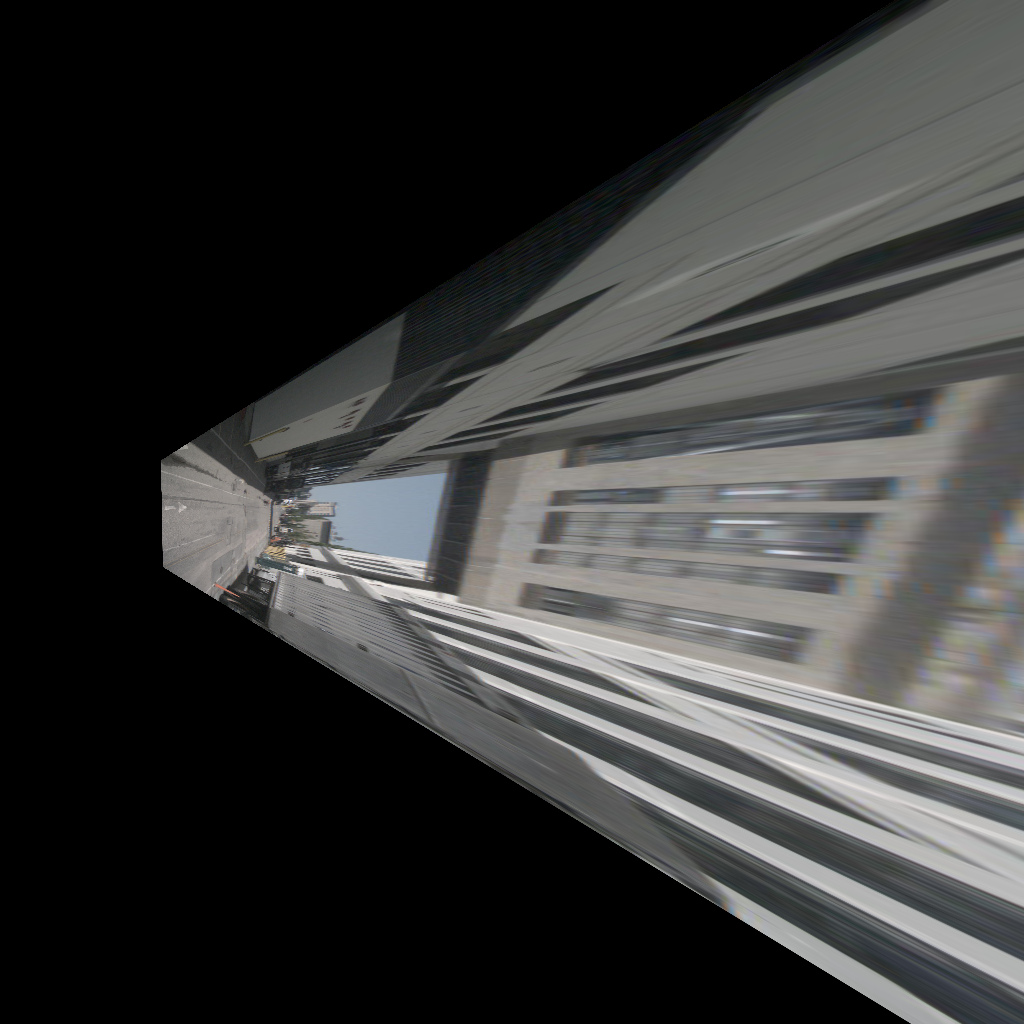
\includegraphics[width=0.15\textwidth]{images/metodology/data_augmentations/rz_-0.25_0.png} & 
        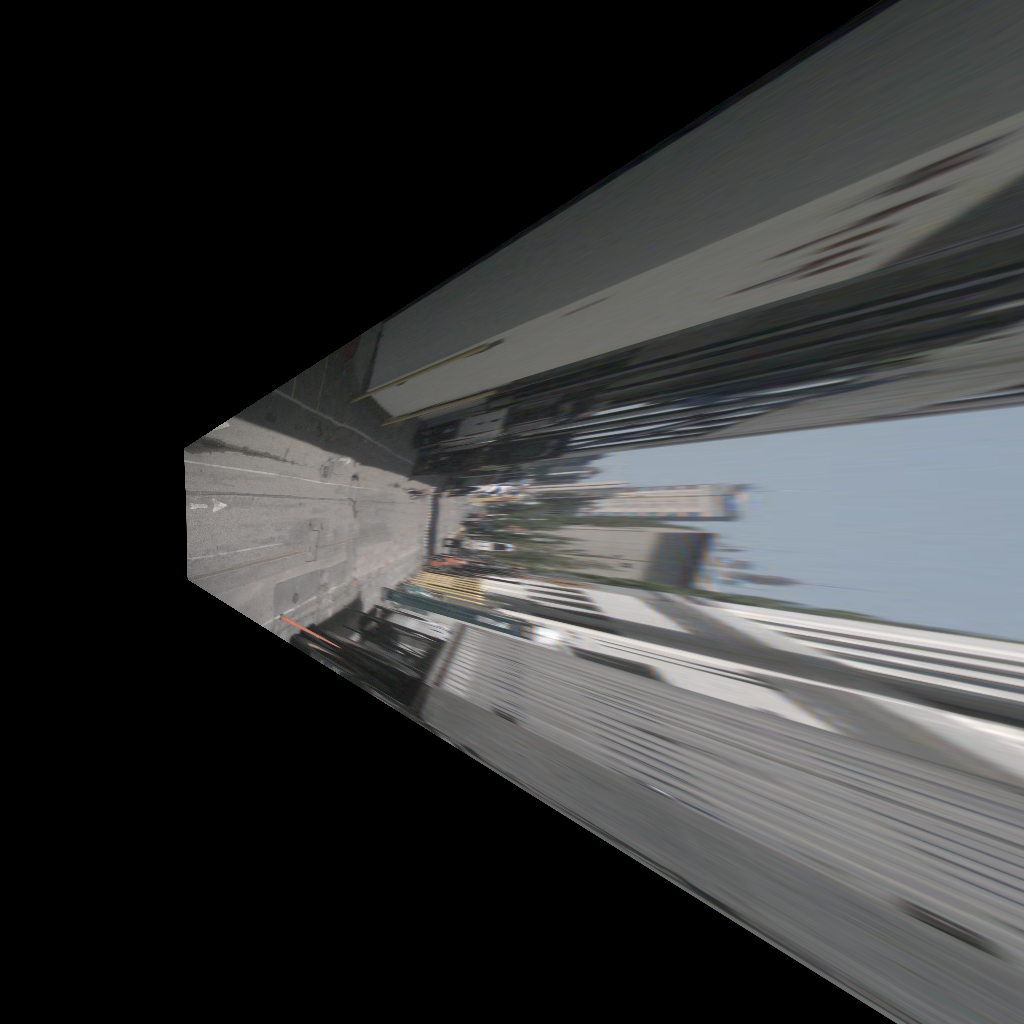
\includegraphics[width=0.15\textwidth]{images/metodology/data_augmentations/rz_-0.125_1.png} & 
        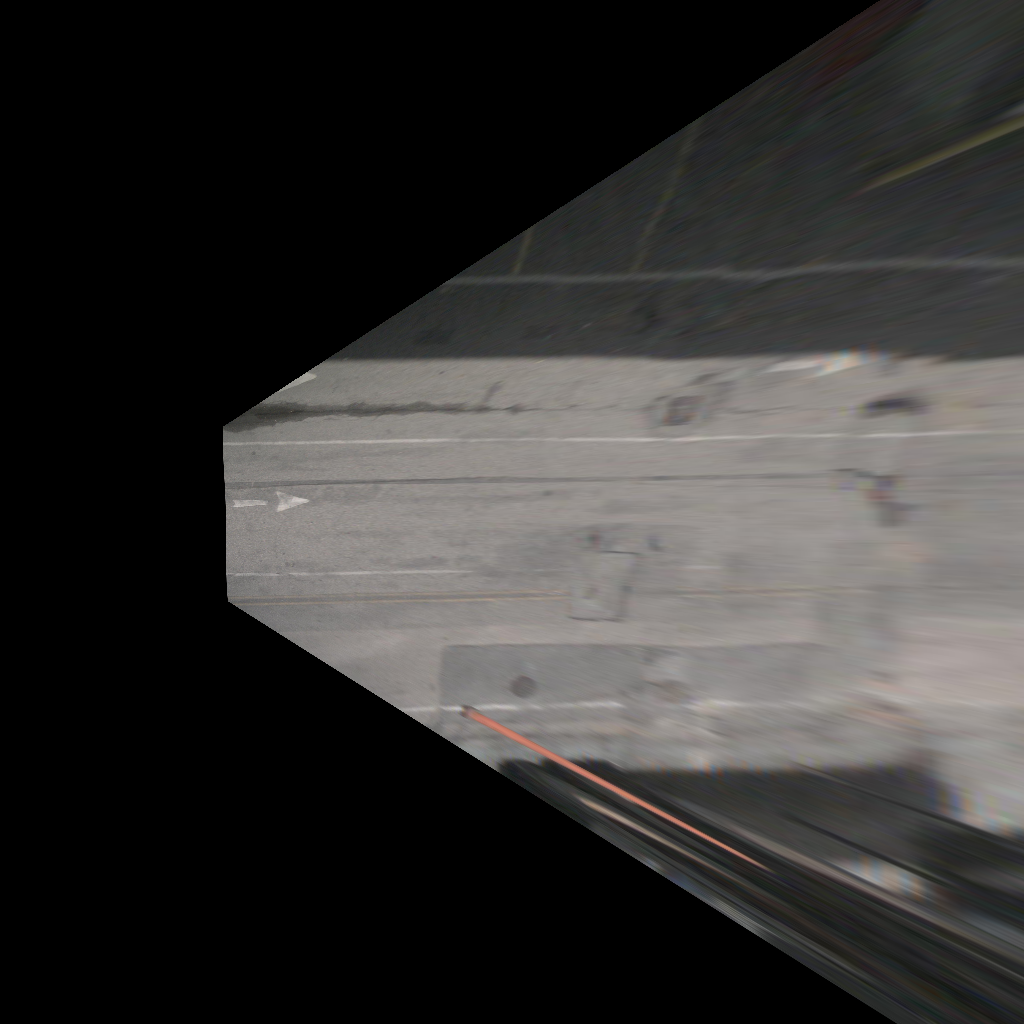
\includegraphics[width=0.15\textwidth]{images/metodology/data_augmentations/rz_0.0_2.png} & 
        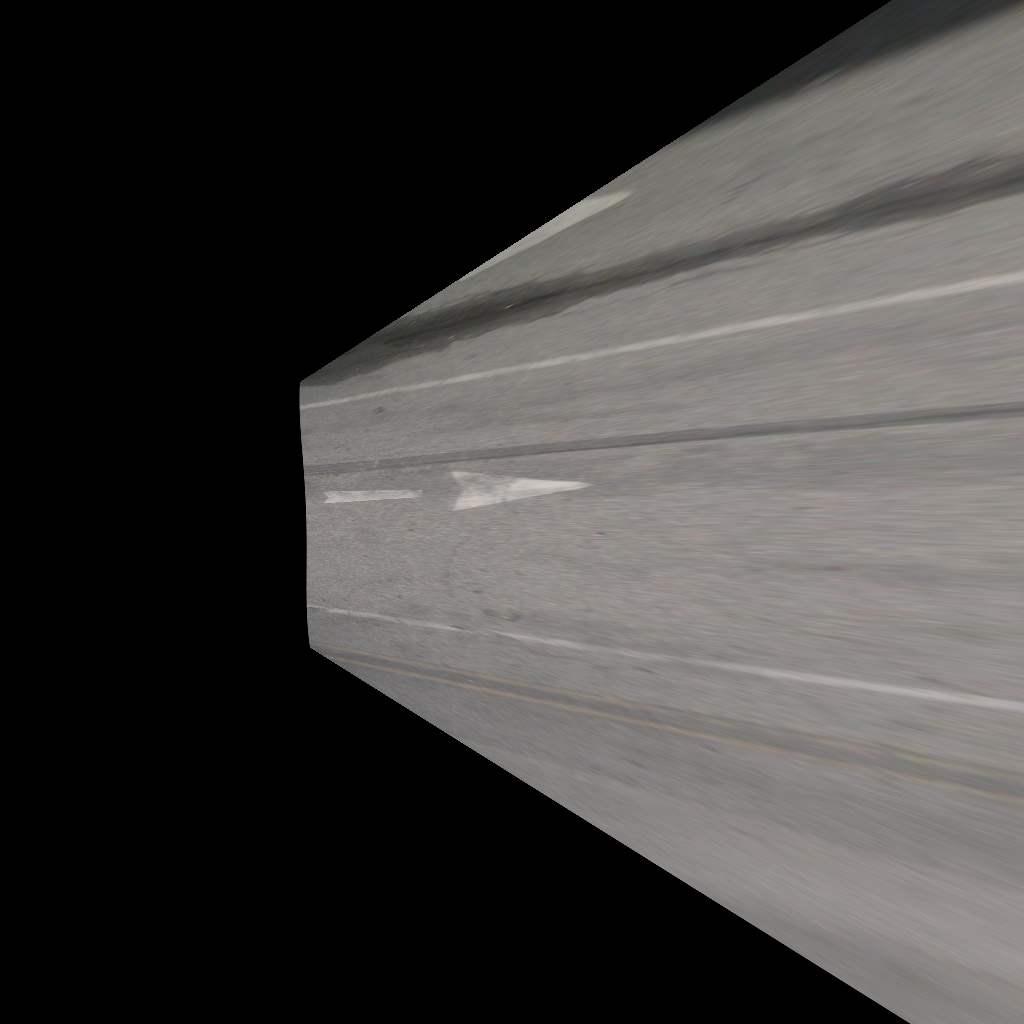
\includegraphics[width=0.15\textwidth]{images/metodology/data_augmentations/rz_0.125_3.png} & 
        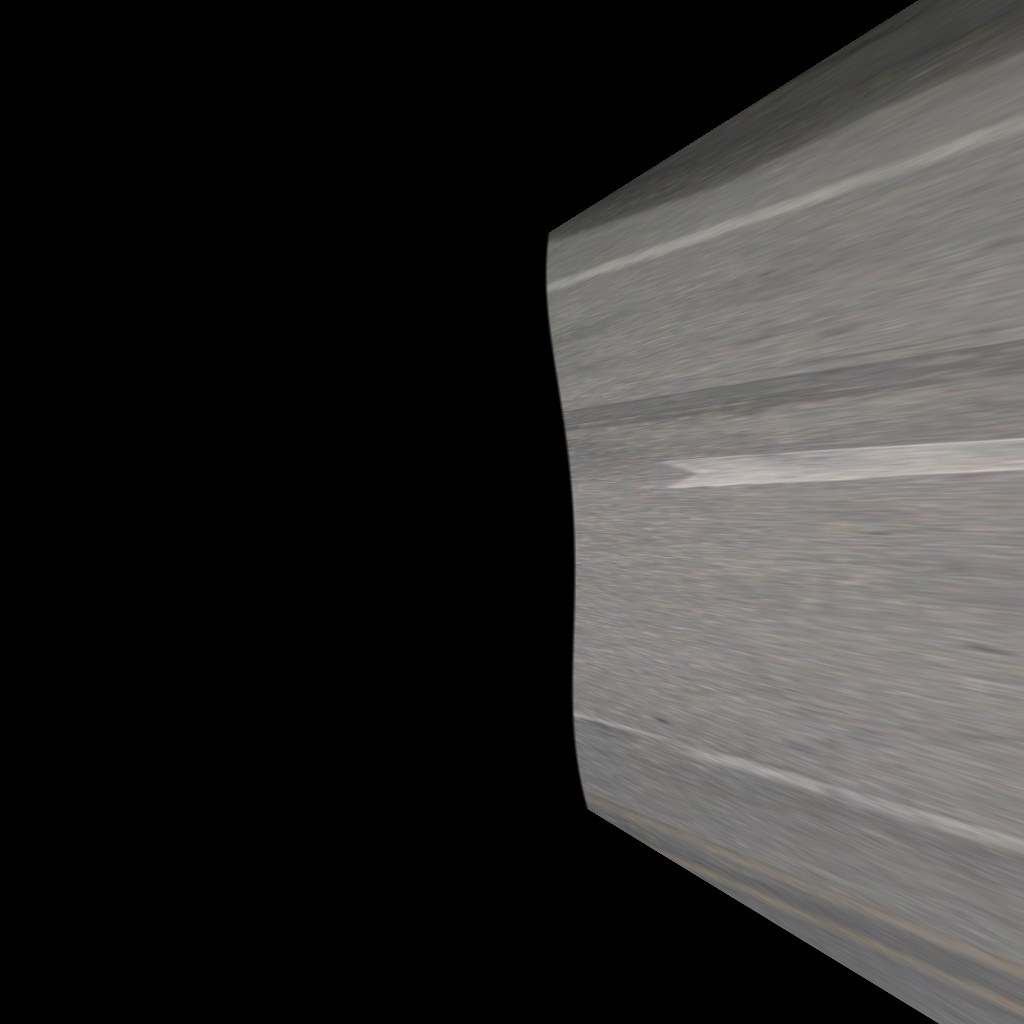
\includegraphics[width=0.15\textwidth]{images/metodology/data_augmentations/rz_0.25_4.png} \\ 

        \rotatebox{90}{\textbf{Roll}} & 
        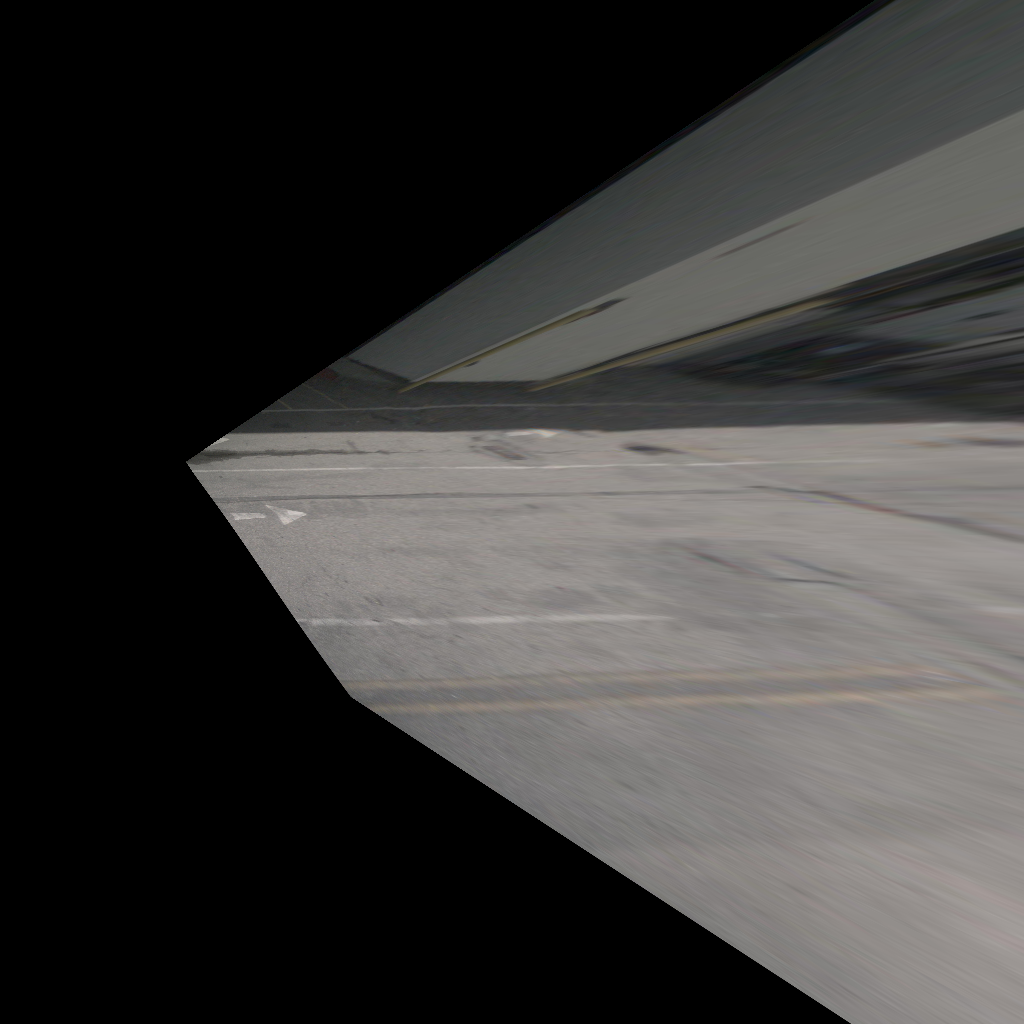
\includegraphics[width=0.15\textwidth]{images/metodology/data_augmentations/ry_-0.25_0.png} & 
        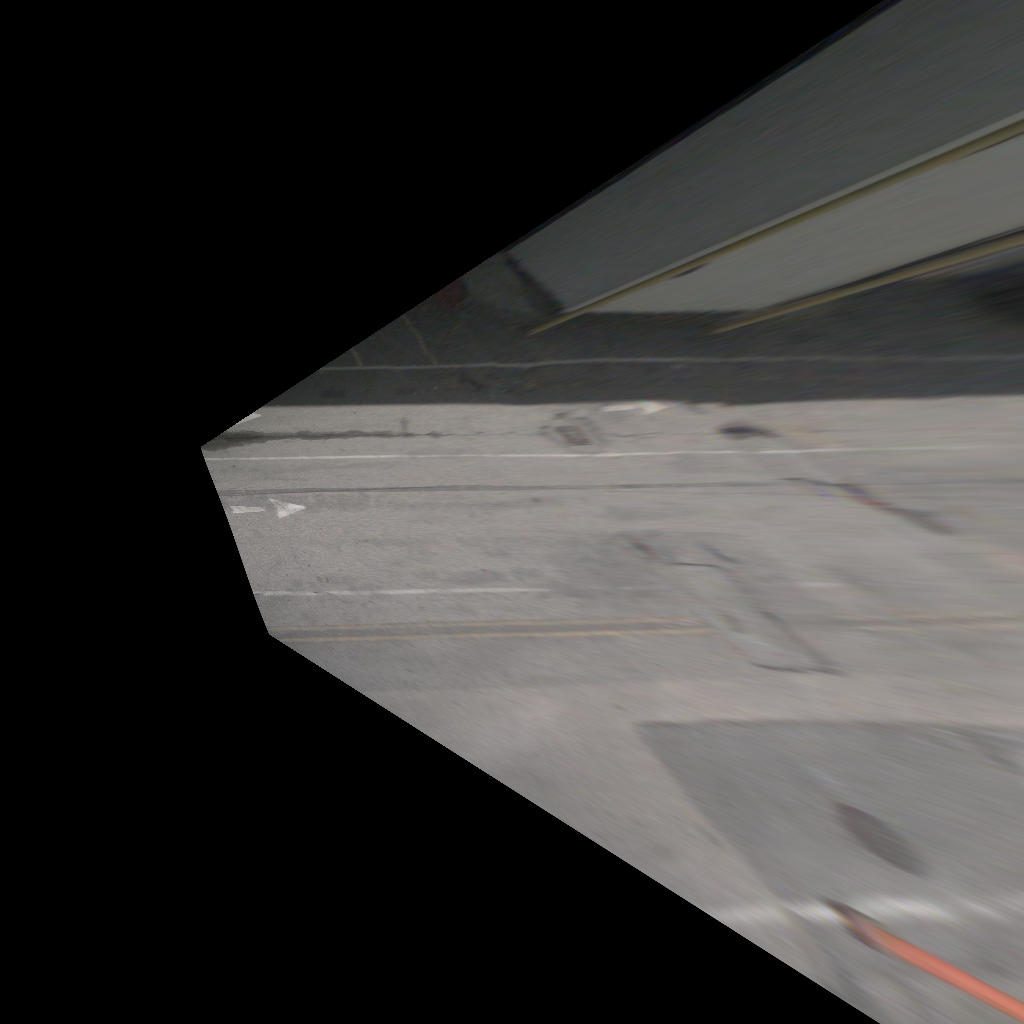
\includegraphics[width=0.15\textwidth]{images/metodology/data_augmentations/ry_-0.125_1.png} & 
        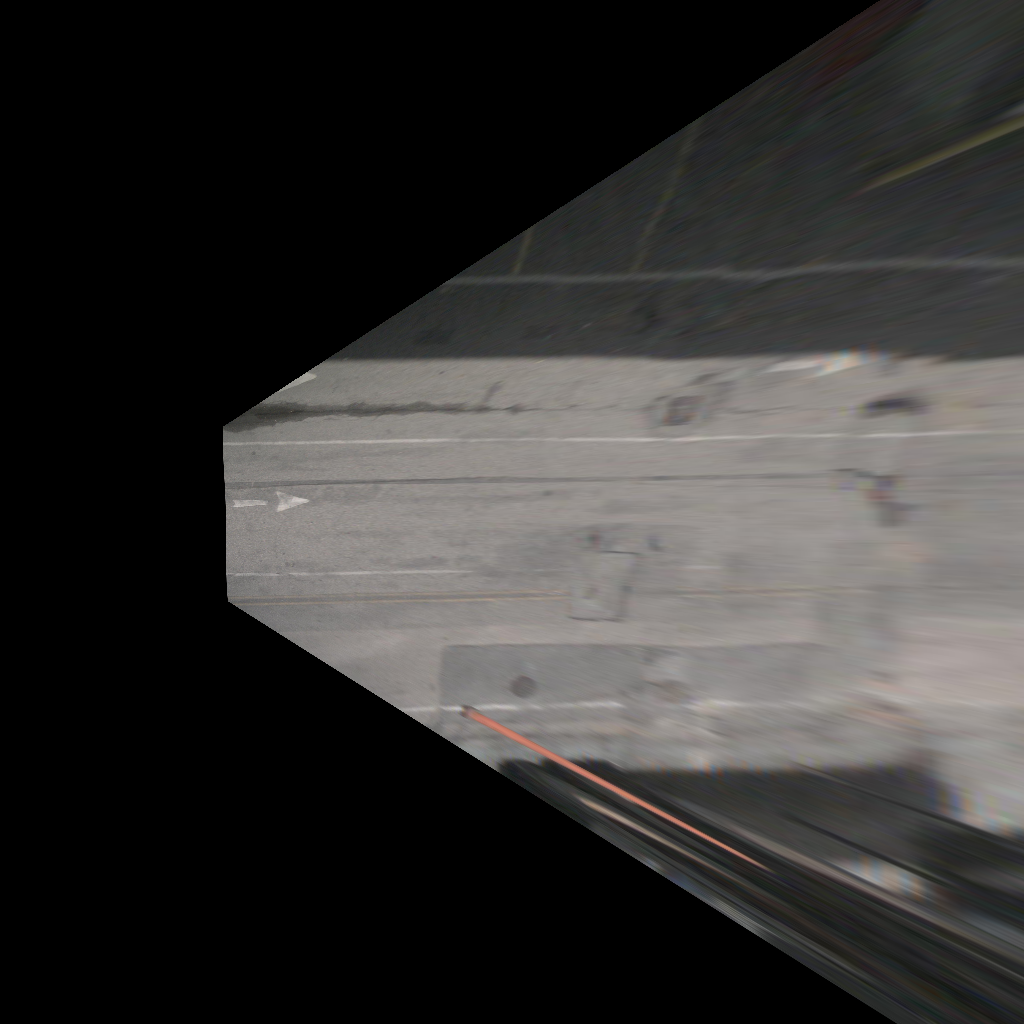
\includegraphics[width=0.15\textwidth]{images/metodology/data_augmentations/ry_0.0_2.png} & 
        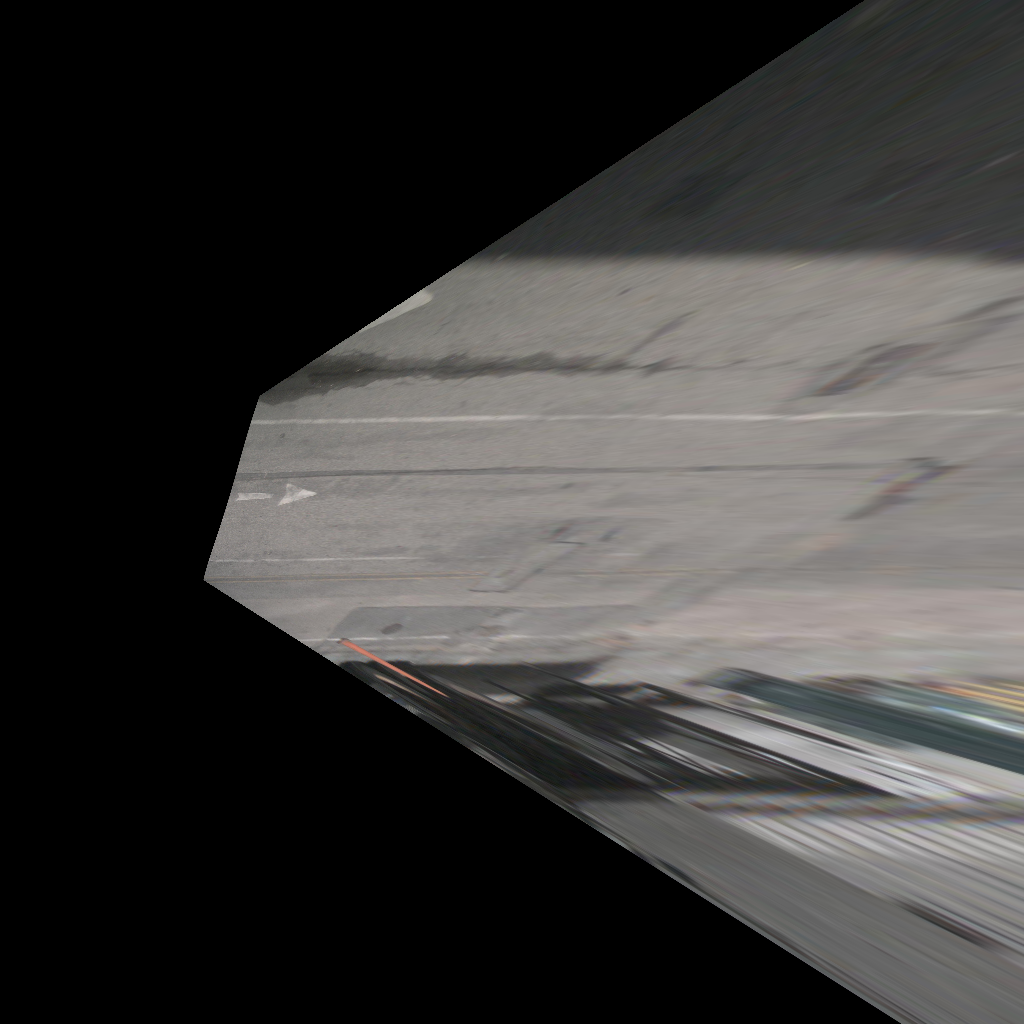
\includegraphics[width=0.15\textwidth]{images/metodology/data_augmentations/ry_0.125_3.png} & 
        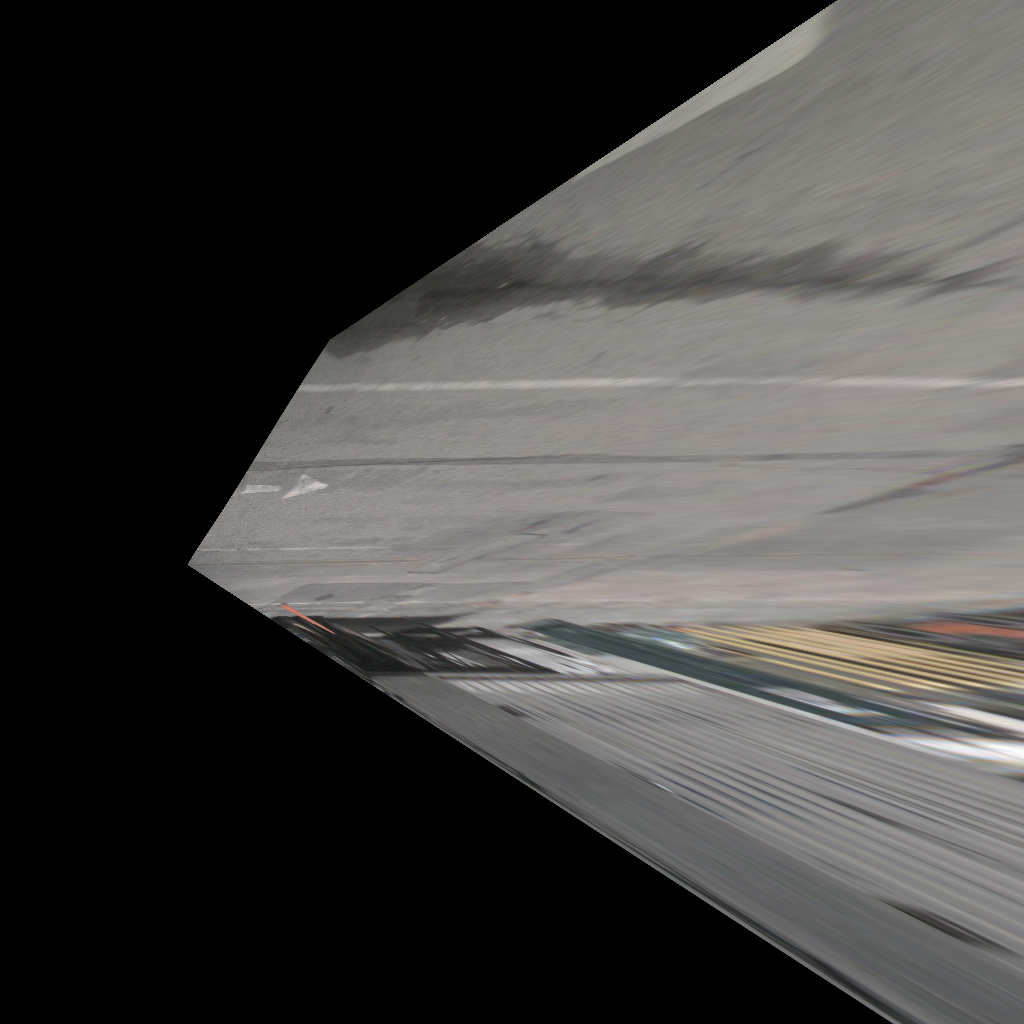
\includegraphics[width=0.15\textwidth]{images/metodology/data_augmentations/ry_0.25_4.png} \\ 
        
    \end{tabular}
    
    \caption{Effect of camera transformations on BEV projection. The first row shows variations in the yaw axis, the second in pitch, and the third in roll.}
    \label{fig:bev_data_aug}
\end{figure}

\hl{This raises an important question: \textit{Which approach is more effective: traditional geometric data augmentation techniques or the modification of extrinsic parameters?}}

\subsubsection{Validation and comparison: Selection module}
Mean intersection over union (mIoU) or Jaccard index is used as the metric for evaluation and comparison between the two approaches.

\hl{Fusion module in the pipeline. Semantic masks are selected from each model depending on its mIoU in the test set?}


\subsection{Driveable area automatic annotation}
\label{aplication}

This section details the selected approach used to automatically annotate occupancy and occlusion masks in vehicular scenes. The method employs a 2D-to-3D approach, using estimated depth maps from monocular images to approximate object dimensions and compute the corresponding masks.

As shown in Figure \ref{fig:application_flow_diagram}, the method can be divided into four main stages: depth estimation, where a depth map is generated from monocular front images; frame point cloud estimation, which creates a 3D representation of the current scene; projection of the perspective semantic mask onto the 3D point cloud to infer object instances for each selected semantic class; and the final computation of occupancy, occluded, and drivable areas by combining 3D object information with BEV semantic masks.

The system's output is annotated in the OpenLABEL format and integrated with the WebLABEL \cite{weblabel} ecosystem, enabling further fine annotations by the user. Additionally, a visualization tool has been developed using the Open3D \cite{open3d} library to facilitate the rendering process of vehicular scenes.

\begin{figure}[h!]
    \centering
    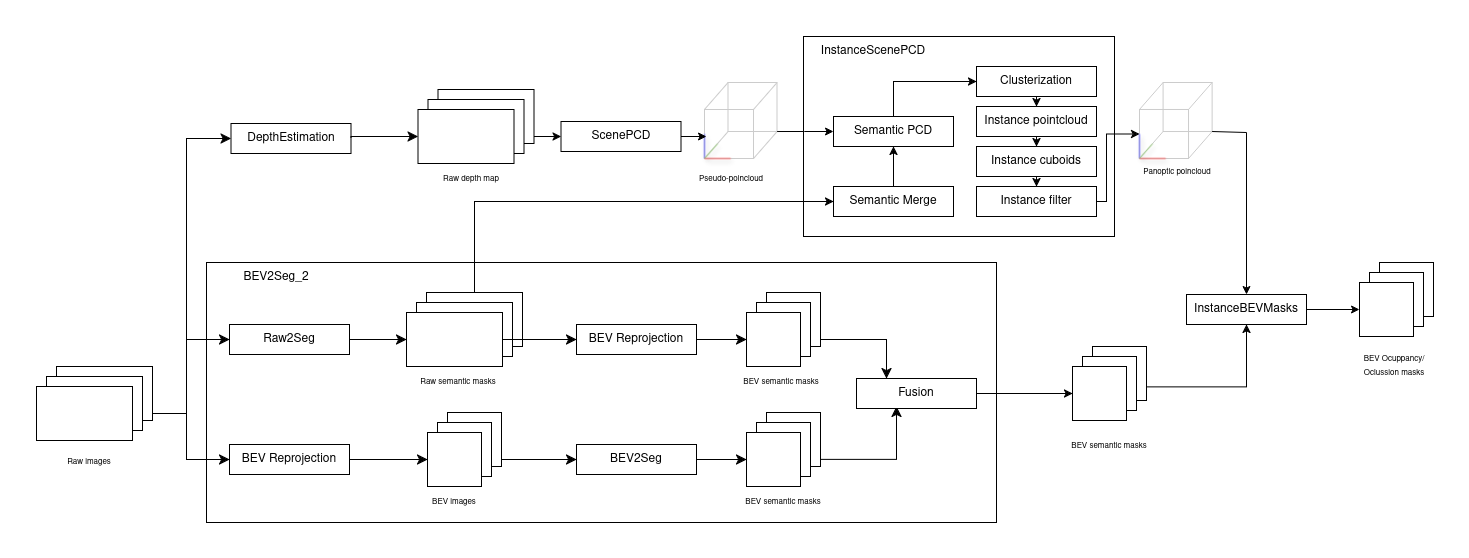
\includegraphics[width=\linewidth]{images/metodology/Application_flow_diagram.png}
    \caption{Annotation flow diagram.}
    \label{fig:application_flow_diagram}
\end{figure}

\subsubsection{Depth estimation}
\label{depth_estimation}


Traditional depth estimation techniques rely on geometric and photometric marks to in


In order to obtain a depth estimation from monocular images, Depth-Pro \cite{depth-pro} has been selected as the estimation model which is " a foundation model for zero-shot metric monocular depth estimation"



\begin{figure}[h]
    \centering
    % Row labels
    \setlength{\tabcolsep}{1pt}  % Reduce column padding
    \renewcommand{\arraystretch}{0.5}
    \begin{tabular}{c c c c c c c c}
        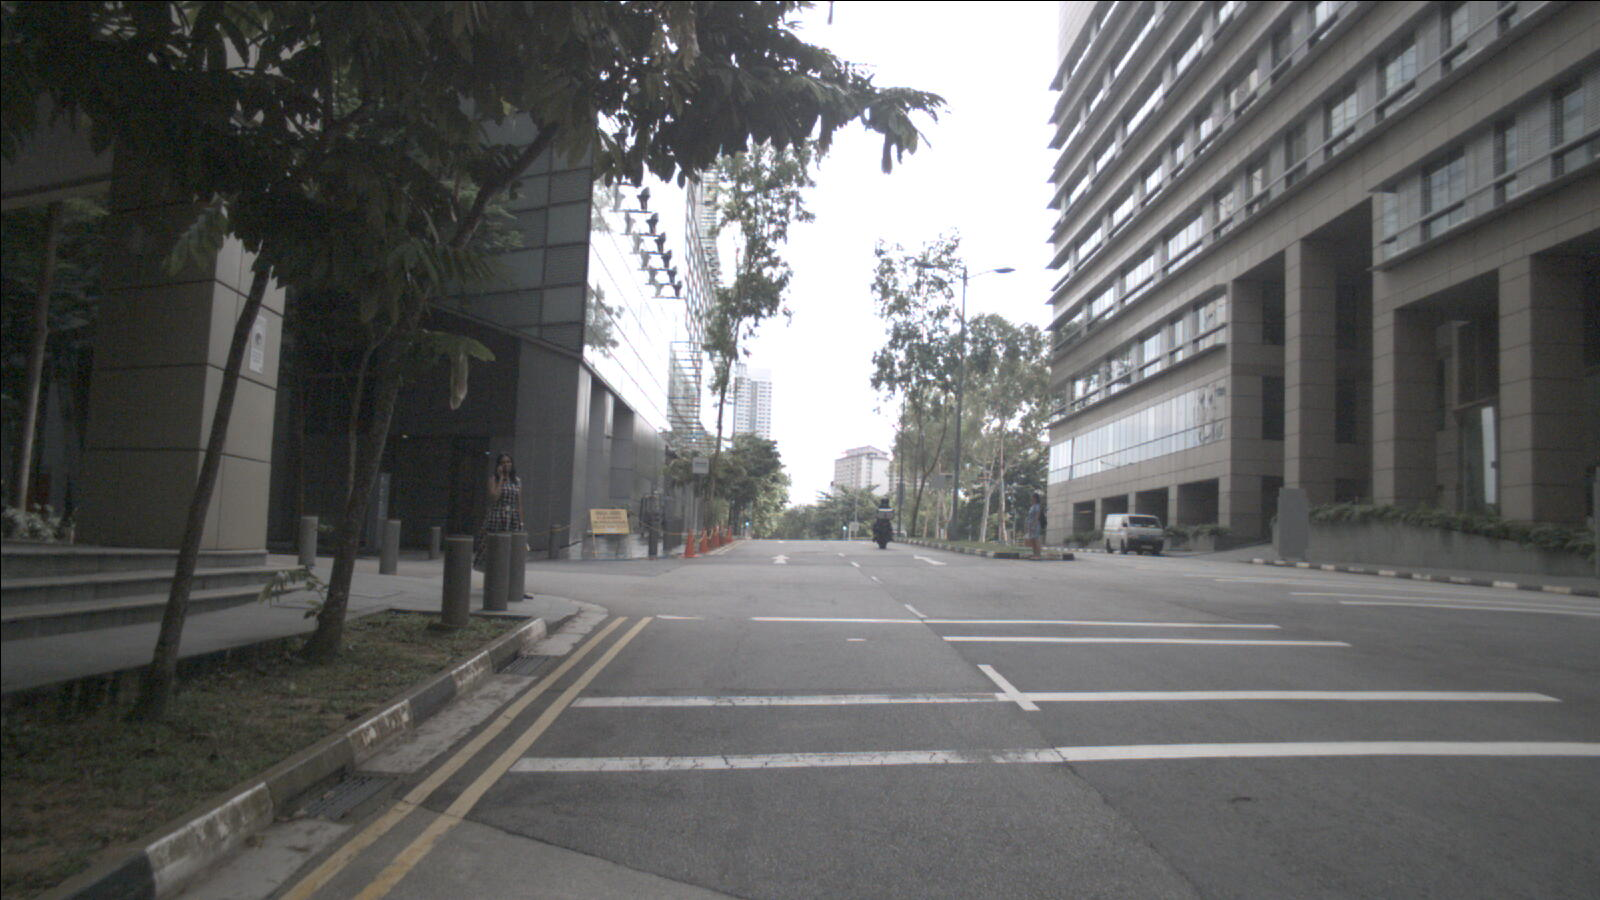
\includegraphics[width=0.12\textwidth]{images/metodology/depth_images/original_image_0.png} & 
        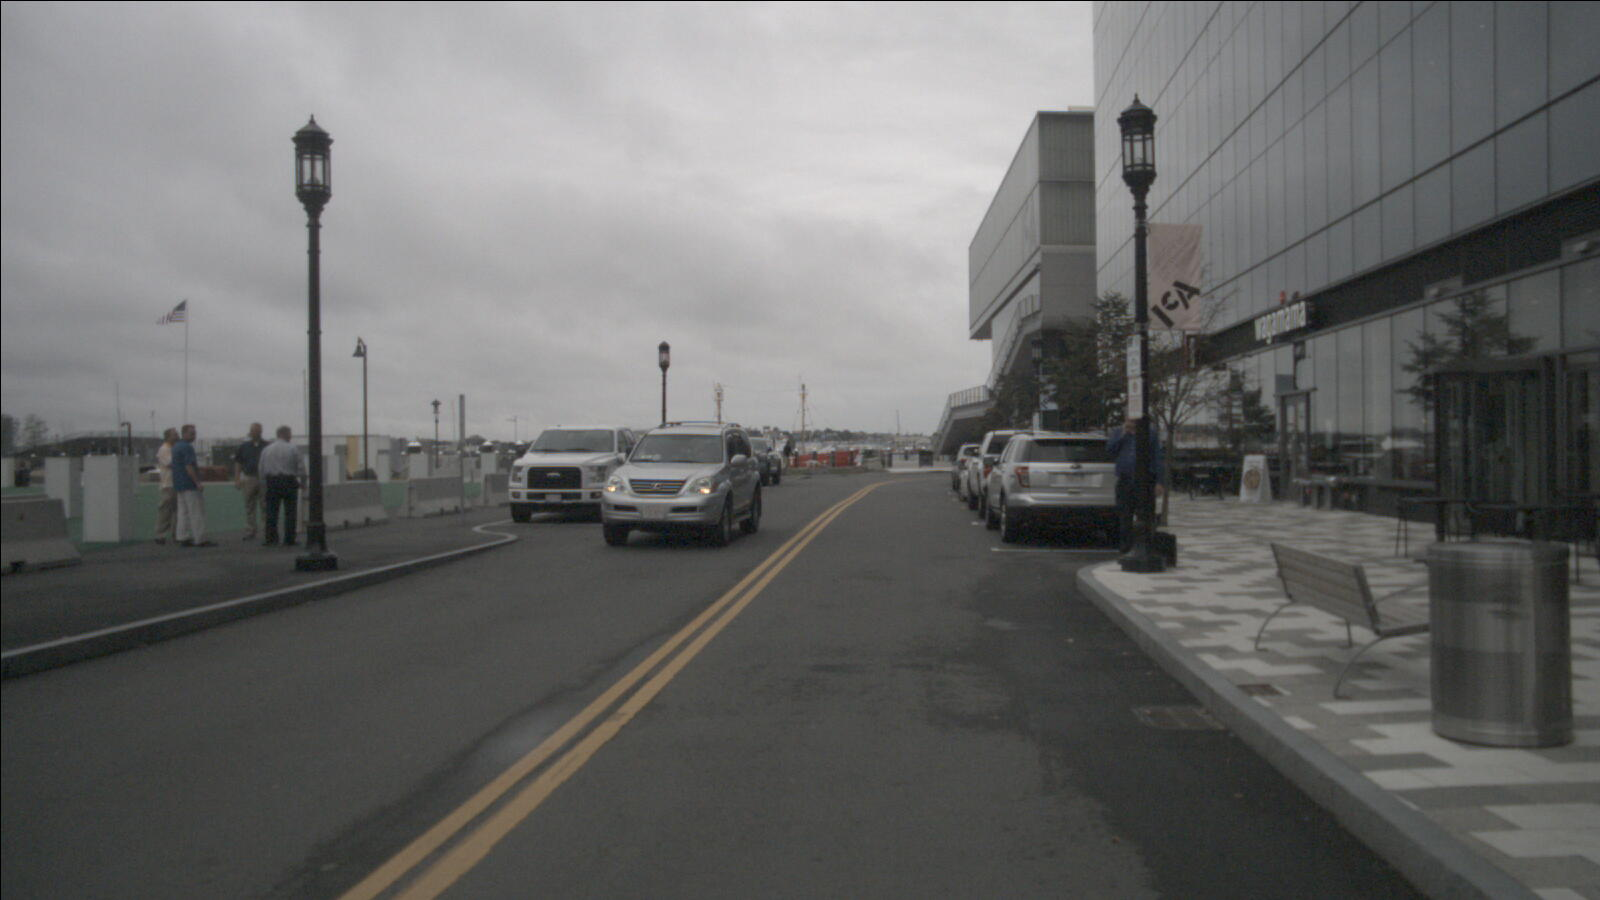
\includegraphics[width=0.12\textwidth]{images/metodology/depth_images/original_image_1.png} & 
        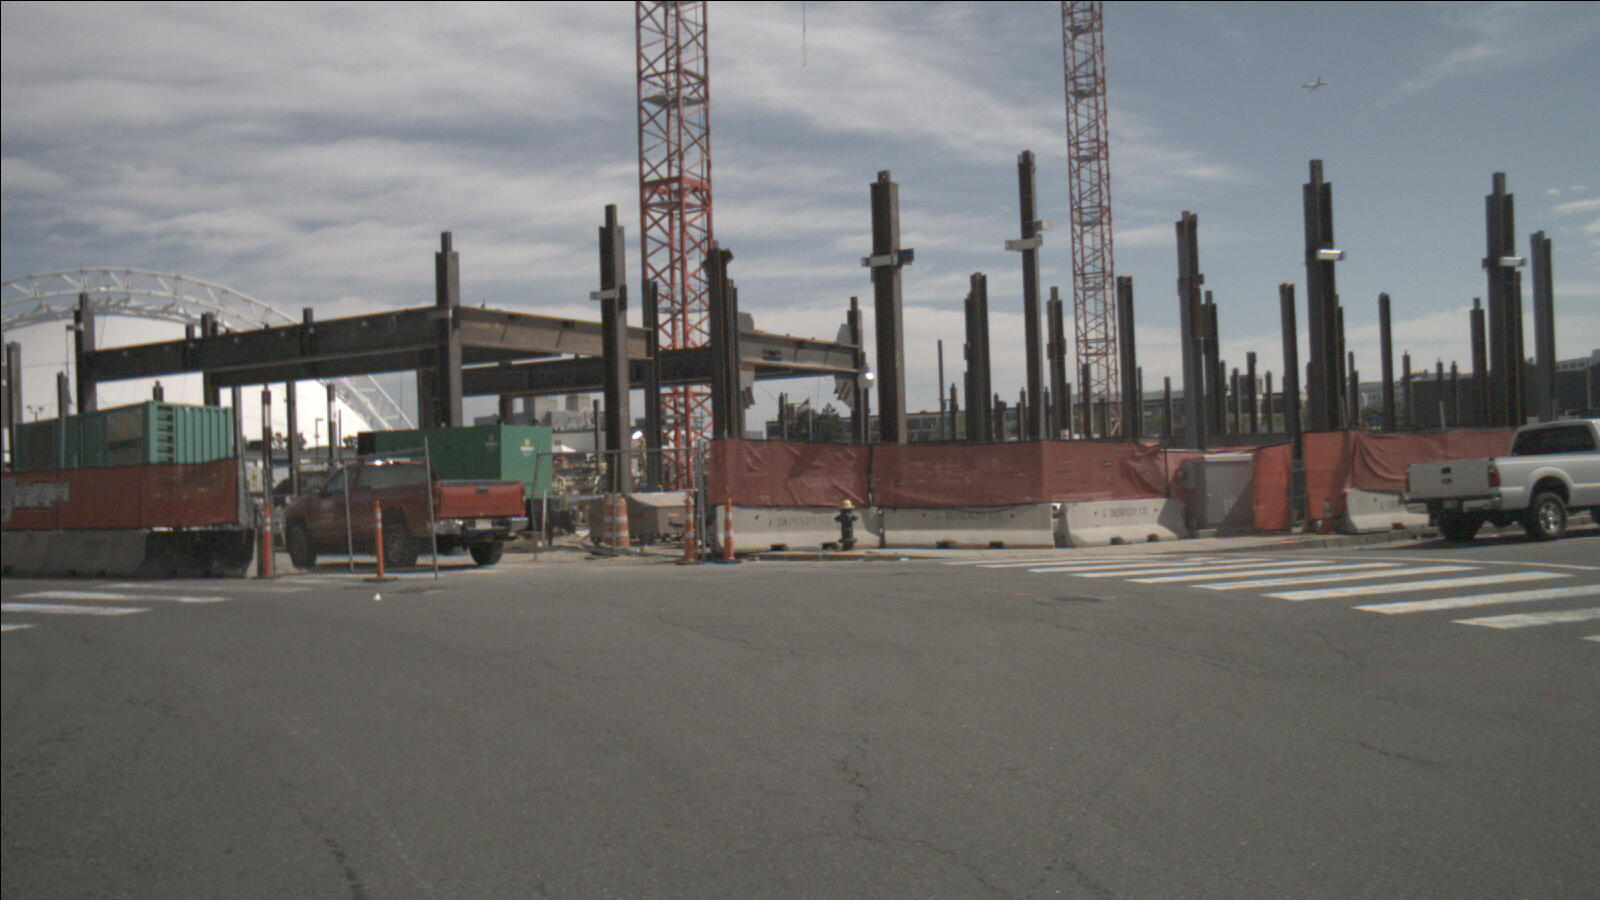
\includegraphics[width=0.12\textwidth]{images/metodology/depth_images/original_image_2.png} &
        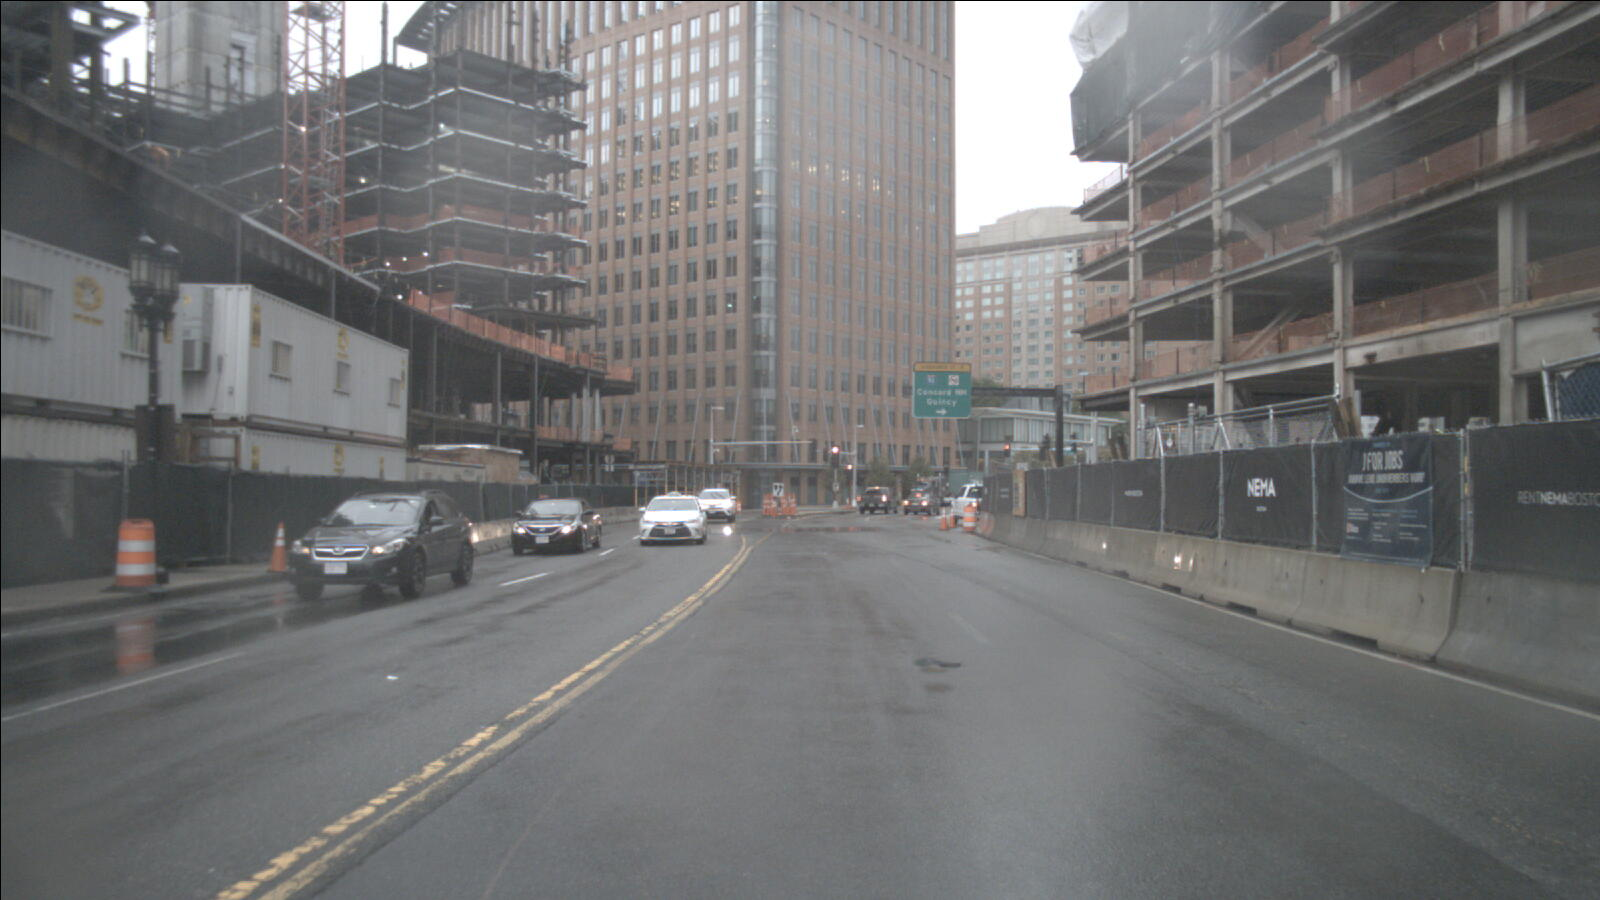
\includegraphics[width=0.12\textwidth]{images/metodology/depth_images/original_image_3.png} &
        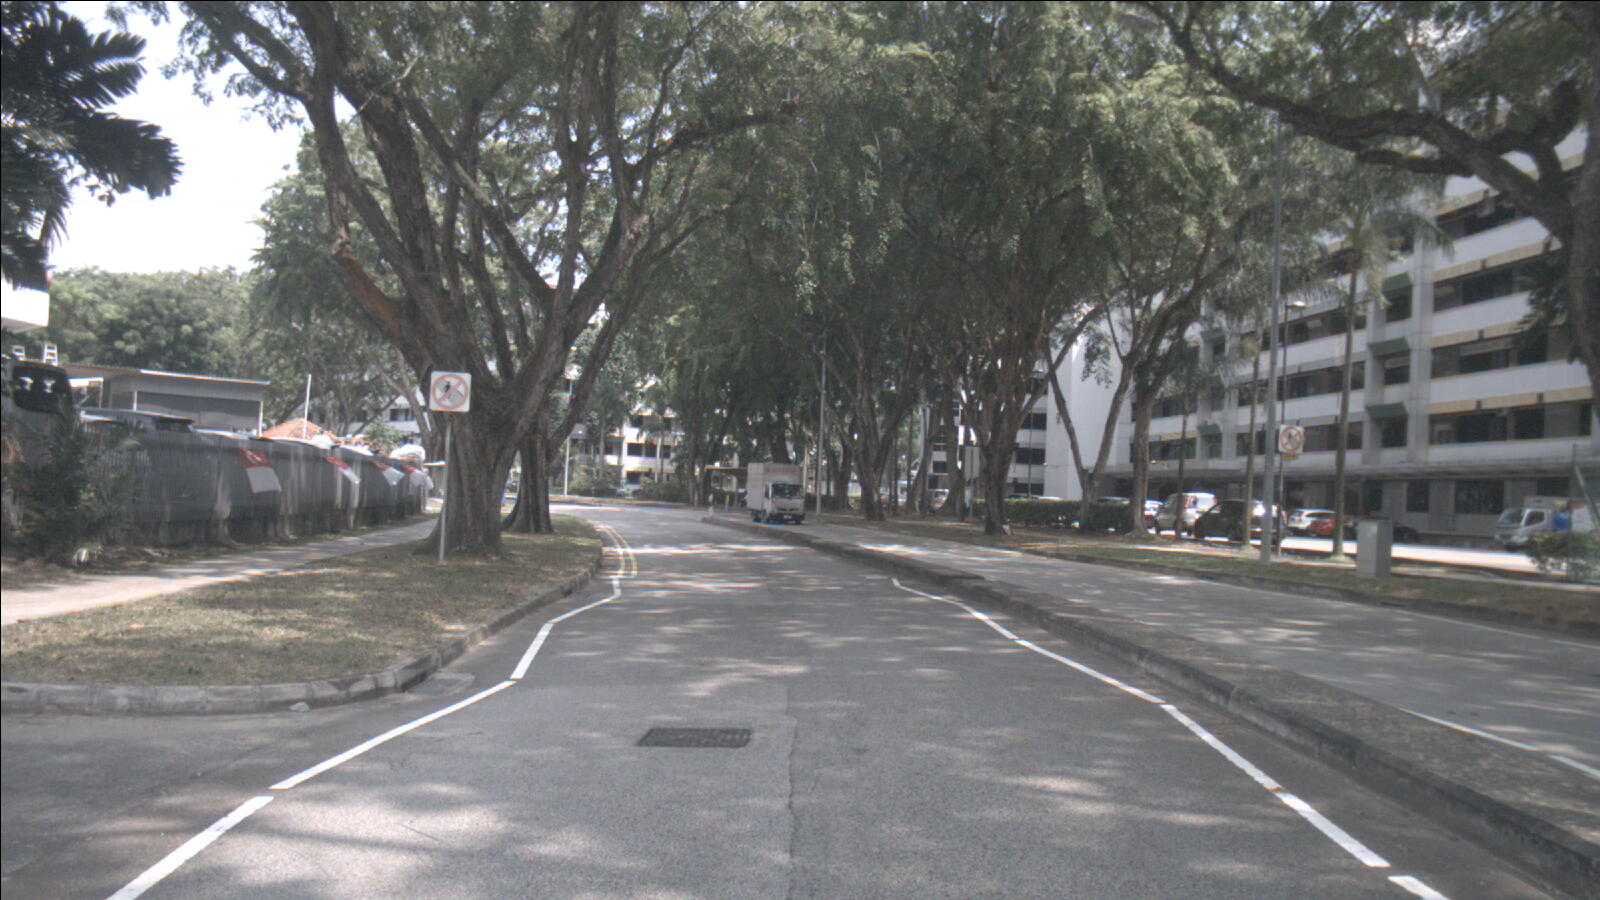
\includegraphics[width=0.12\textwidth]{images/metodology/depth_images/original_image_4.png} &   
        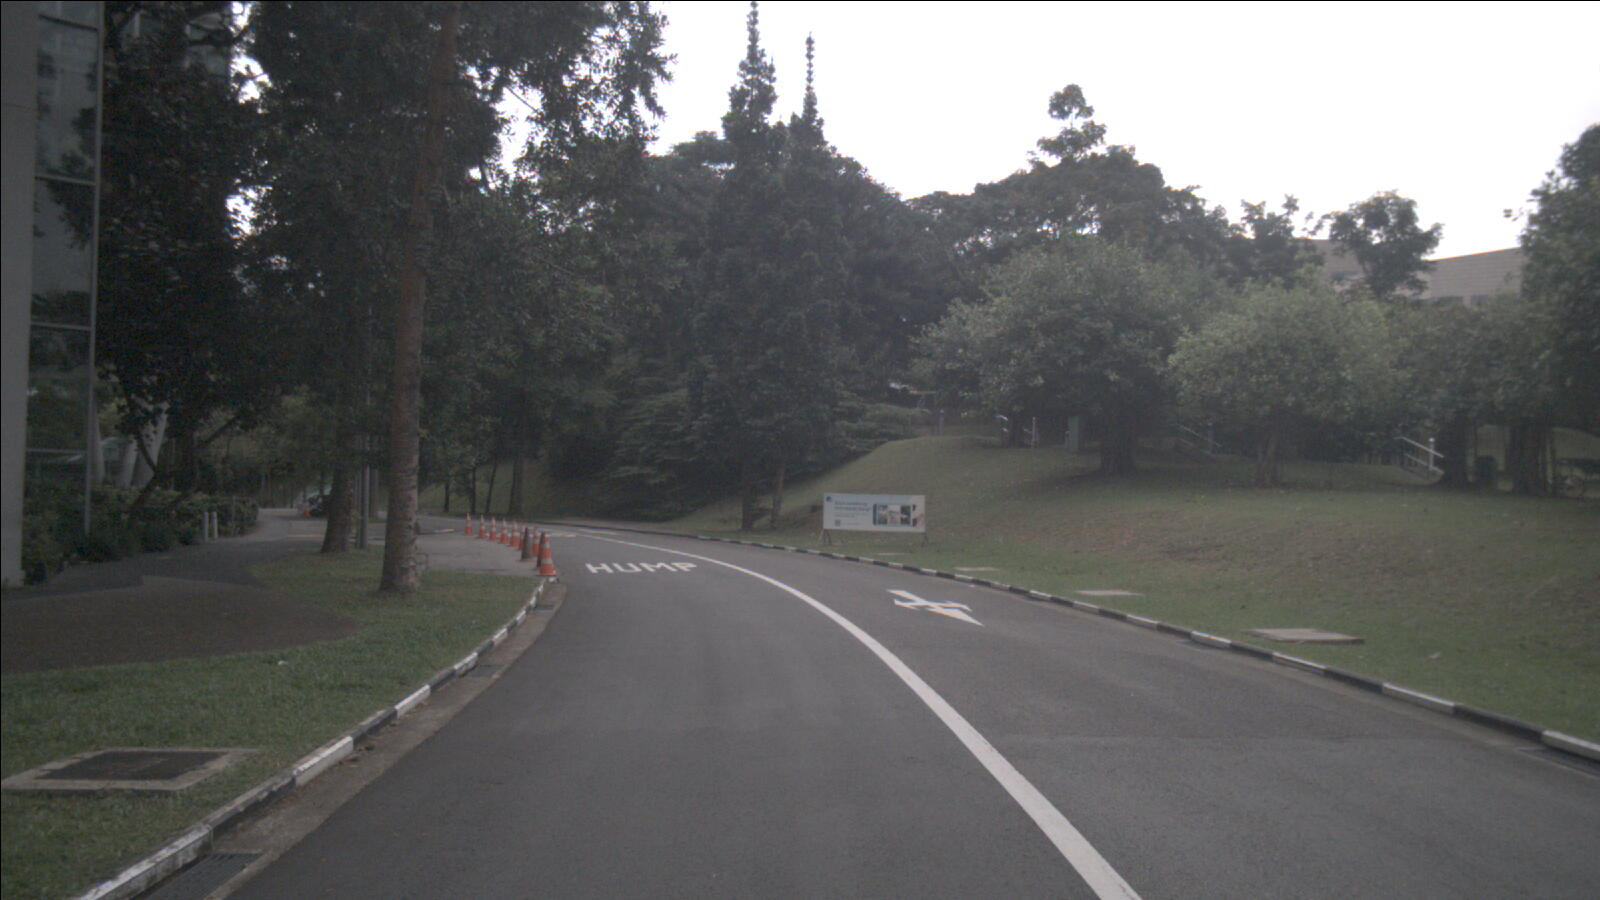
\includegraphics[width=0.12\textwidth]{images/metodology/depth_images/original_image_5.png} & 
        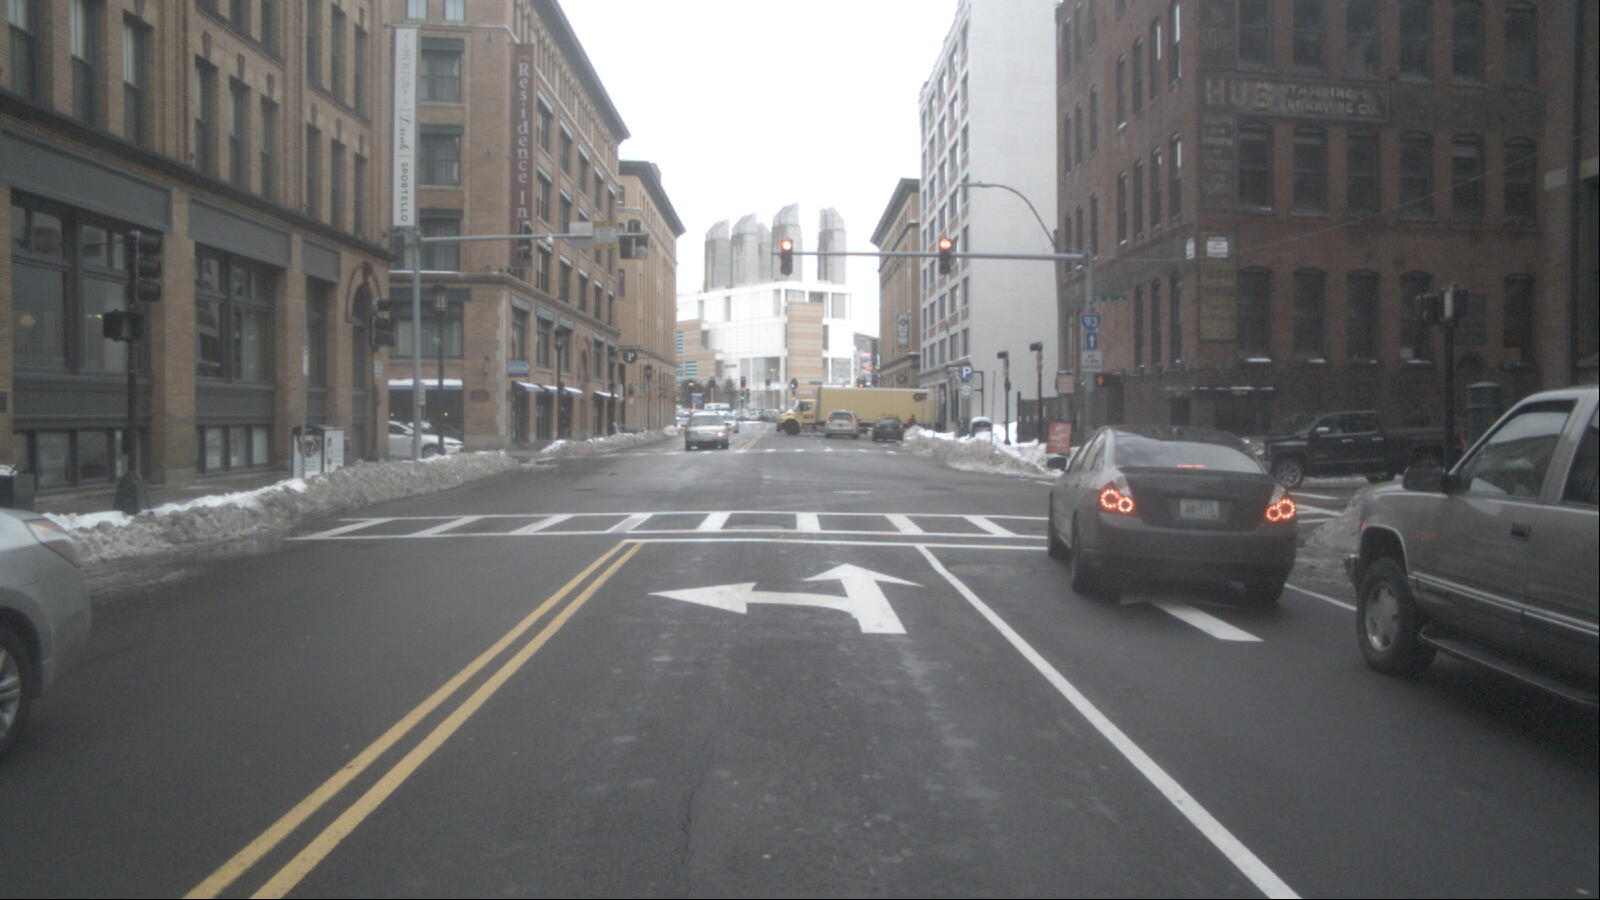
\includegraphics[width=0.12\textwidth]{images/metodology/depth_images/original_image_6.png} &
        \includegraphics[width=0.12\textwidth]{images/metodology/depth_images/original_image_7.png} \\

        \includegraphics[width=0.12\textwidth]{images/metodology/depth_images/colored_depth_map_0.png} & 
        \includegraphics[width=0.12\textwidth]{images/metodology/depth_images/colored_depth_map_1.png} & 
        \includegraphics[width=0.12\textwidth]{images/metodology/depth_images/colored_depth_map_2.png} &
        \includegraphics[width=0.12\textwidth]{images/metodology/depth_images/colored_depth_map_3.png} &
        \includegraphics[width=0.12\textwidth]{images/metodology/depth_images/colored_depth_map_4.png} &   
        \includegraphics[width=0.12\textwidth]{images/metodology/depth_images/colored_depth_map_5.png} & 
        \includegraphics[width=0.12\textwidth]{images/metodology/depth_images/colored_depth_map_6.png} &
        \includegraphics[width=0.12\textwidth]{images/metodology/depth_images/colored_depth_map_7.png} \\
    \end{tabular}    
    \caption{Depht maps estimated with Depth-Pro model.}
    \label{fig:depth_images}
\end{figure}

\subsubsection{Scene PCD}
When an image is captured, the 3D geometry of the scene is projected onto a 2D representation, which is then rasterized into the pixel space of the image. This transformation from 3D world coordinates to 2D image coordinates is known as the \emph{camera projection process}. In its simplest form, this is described by the \emph{pinhole camera model}, illustrated in Figure \ref{fig:pinhole_model}. In this setup, $\mathbf{O}_w$ represents the world coordinate frame, $\mathbf{F}_c$ denotes the camera coordinate frame (typically located at the camera's optical center or pinhole), and $\mathbf{F}_i$ defines the 2D image plane.

\begin{figure}[h!]
    \centering
    \includegraphics[width=\linewidth]{images/shared/no_signal.jpg}
    \caption{Ideal perspective camera model.}
    \label{fig:pinhole_model}
\end{figure}

Starting with a 3D point expressed in world coordinates, $\mathbf{P}_w = \left(x_w, y_w, z_w\right)^\top$, the point can be transformed int the camera coordinate frame using a rotation matrix $\mathbf{R}$ and a translation vector $\mathbf{t}$. These are known as camera's extrinsic parameters and are commonly combined into a single homogeneous transformation matrix denoted as $\left[\mathbf{R} \,|\, \mathbf{t}\right]$.

\begin{align}
    \tilde{\mathbf{P}}_c 
    &=
    \begin{pmatrix}
        x_c \\
        y_c \\
        z_c \\
        1
    \end{pmatrix}
    =
    \begin{pmatrix}
        r_{11} & r_{12} & r_{13} & t_x \\
        r_{21} & r_{22} & r_{23} & t_y \\
        r_{31} & r_{32} & r_{33} & t_z \\
        0 & 0 & 0 & 1
    \end{pmatrix}
    \begin{pmatrix}
        x_w \\
        y_w \\
        z_w \\
        1
    \end{pmatrix}
    =
    \left[ \mathbf{R} \,|\, \mathbf{t} \right] \tilde{\mathbf{P}}_w 
\end{align}

Once the point is expressed in the camera coordinate frame $\mathbf{F}_c$, it is projected onto the image plane $\mathbf{F}_i$ using the intrinsic parameters of the camera, which describe how the 3D geometry of the scene is mapped to the 2D image sensor. Under the pinhole camera model, this projection involves a perspective division (to normalize the coordinates) followed by a transformation using the intrinsic matrix $\mathbf{K}$, which encodes the focal lengths and maps the continuous 2D space to the discrete pixel grid of the digital camera, while also considering the sensor's displacement of the principal point $(c_x, c_y)$. The final pixel coordinates can be computed as:

\begin{align}
    \tilde{\mathbf{p}_i}
    = \left(u, v, 1\right)^\top
    = \mathbf{K} \cdot \frac{1}{z_c} \tilde{\mathbf{P}}_c
\end{align}

where $\mathbf{K}$ is the intrinsic calibration matrix, typically given by:

\begin{align}
    \mathbf{K} =
    \begin{pmatrix}
        f_x & 0 & c_x \\
        0 & f_y & c_y \\
        0 & 0 & 1
    \end{pmatrix}
\end{align}

Here, $f_x$ and $f_y$ are the focal lengths in pixel units along the $\hat{x}_i$ and $\hat{y}_i$ axes.

However, the images used in this thesis are taken from lens-cameras which introduces inherent tangential and radial distorsions which are taken into consideration by rectifying the camera normalized 3D points before appying the camera's intrinsic matrix $\mathbf{K}$.

Despite all of this, the objective of this module is to make the inverse process of computing the scene pointcloud starting from points in the pixel domain. This is known as reprojection and has the challenging task of infering a third 3D dimension which were lost during the image capturing process. To address this, the depht map $D_{h \times w}$ of the image is estimated \ref{depth_estimation} and the camera parameters are known. 

The approach employed for this task is represented in Algorithm \ref{algorithm:scene_pcd_hloop} where the 3D points of the image are calculated for each image column. The resulting dense pointcloud can be seen in Figure \ref{fig:pcd_scene_images}.

In order to compute the scene pointcloud given an image $I_{h \times w}$ and it's corresponding depth map $D_{h \times w}$ and the intrinsics parameters of the camera $K$ it is prety straight forward. 

\hl{mention that the h-loop strategy was selected as it has greater performance.}

\begin{algorithm}
    \caption{Pointcloud calculation}
    \label{algorithm:scene_pcd_hloop}
    \footnotesize

    \begin{algorithmic}[1]
        \State \textbf{Input:} Depth map $D_{\left[h \times w\right]}$, camera intrinsics $K$ 
        \State \textbf{Output:} Pointcloud $P^{raw}_{\left[3 \times h \times w\right]}$
        
        \State Initialize $P_{\left[3 \times h \times w\right]} \gets \mathbf{0}$

        \For{$i \text{ in } \left[0, 1, \dots, h-1\right]$}
            \State $pix\_coords_{3 \times w} \gets \begin{bmatrix} \text{0:w-1} & \mathbf{i}_w & \mathbf{1}_w \end{bmatrix}$
            \State $cam\_rays_{3 \times w} \gets K^{-1} \cdot pix\_coords$
            
            \State $P^{raw}[:, i, :] \gets cam\_rays[2, :] \cdot D[i, :]$  \Comment{Update the $i$-th row of $P$. The ray's z-value is the depht}
        \EndFor
        
        \State \Return $P^{raw}$
    \end{algorithmic}
\end{algorithm}

\begin{figure}[h]
    \centering
    % Row labels
    \setlength{\tabcolsep}{1pt}  % Reduce column padding
    \renewcommand{\arraystretch}{0.5}
    \begin{tabular}{c c c c c c c c}
        \includegraphics[width=0.12\textwidth]{images/metodology/pcd_images/frame_0.png} & 
        \includegraphics[width=0.12\textwidth]{images/metodology/pcd_images/frame_1.png} & 
        \includegraphics[width=0.12\textwidth]{images/metodology/pcd_images/frame_2.png} &
        \includegraphics[width=0.12\textwidth]{images/metodology/pcd_images/frame_3.png} &
        \includegraphics[width=0.12\textwidth]{images/metodology/pcd_images/frame_4.png} &   
        \includegraphics[width=0.12\textwidth]{images/metodology/pcd_images/frame_5.png} & 
        \includegraphics[width=0.12\textwidth]{images/metodology/pcd_images/frame_6.png} &
        \includegraphics[width=0.12\textwidth]{images/metodology/pcd_images/frame_7.png} \\

    \end{tabular}    
    \caption{Poinclouds.}
    \label{fig:pcd_scene_images}
\end{figure}

\subsubsection{Instance scene PCD}
The objective of this module is to compute an intance pcd from the already computed pointcloud of the scene and the correspondin semantic mask of the input perspective image taken from the BEV2Seg\_2 module \ref{bev2seg_2}. This data gets feeded into the module and a instance differenciation for certain classes is performed, allowing to isolate instance pointclouds and to compute their enclosing cuboids. The resulting panoptic pointcloud would serve as input for future modules and contains the 3D object detection of the scene starting from just a monocular image.

The input semantic mask is preprocessed with a label merging process for merging into the same class simmilar labels. With this process, some ambiguities and similar label preddictions of the model are mitigated to reduce noise which would affect the following instance estimation processes. The merging policy is default defined as follows and as it can be seen, the target class "vehicle.car" represents all NuScenes vehicles similar to cars.

% DEFAULT_MERGE_DICT = { 'vehicle.car': [     "vehicle.bus.bendy",      "vehicle.bus.rigid",      "vehicle.car",      "vehicle.construction",      "vehicle.emergency.ambulance",      "vehicle.emergency.police",      "vehicle.trailer",      "vehicle.truck" ], "vehicle.motorcycle":[     "vehicle.bicycle",     "vehicle.motorcycle" ] }

Once the semantic mask is preprocessed and the computed pointcloud is computed, a pre-filtering process is performed to remove those points out of some bounds (by default $\left[10, 5, 30\right]$ meters in $x$, $y$ and $z$). Then, the semantic mask is projected into the pointcloud to obtain a semantic pointcloud. This is pretty straight forward as each 3D point is accessed with the same indices for its corresponding pixel semantic label. With this process, each semantic label has its corresponding pointcloud associated.

\hl{Include a Figure of this results}

Also, each semantic pointcloud is marked with a 'dynamic' flag which relates each semantic class with if the object may move or not. Only semantic pointclouds with this label setted gets pass throught the instance detection process. This is to avoid performing those process on labels like background, road barriers, driveable area...

% Finally, a clusterization algorithm is used to extract the different instances of each dynamic semantic pointcloud. The selected algorithm is DBSCAN \footnote{\url{https://scikit-learn.org/stable/modules/generated/sklearn.cluster.DBSCAN.html#sklearn.cluster.DBSCAN}} which creates good instance clusters and removes part of the trail left by the depht estimation on object edges.

With this, for each computed instance pointcloud, the minimal containing oriented 3D bounding boxes are calculated using the Jylanki algorithm.

Finally, a filtering process is made to ensure there are no noisy instances, redundant instances, or too far away or floating instances.


\begin{algorithm}
    \caption{Instance filtering}
    \label{algorithm:instance_filter}
    \footnotesize

    \begin{algorithmic}[1]
        \State \textbf{Input:} $P^{inst}$ panoptic pointcloud
        \State \textbf{Output:} $P^{inst}$ filtered panoptic pointcloud
        
        \For{$label \text{ in } P^{inst}$}
            \For{$i \text{ in } P^{inst}\left[label\right]$}
                \State $B \gets $
            
            \EndFor
        \EndFor
        
        \State \Return $P$
    \end{algorithmic}
\end{algorithm}



\begin{figure}[h]
    \centering
    % Row labels
    \setlength{\tabcolsep}{1pt}  % Reduce column padding
    \renewcommand{\arraystretch}{0.5}
    \begin{tabular}{c c c c c c c c}
        \includegraphics[width=0.12\textwidth]{images/metodology/raw_cuboids/raw_cuboid_1.png} & 
        \includegraphics[width=0.12\textwidth]{images/metodology/raw_cuboids/raw_cuboid_2.png} & 
        \includegraphics[width=0.12\textwidth]{images/metodology/raw_cuboids/raw_cuboid_4.png} &
        \includegraphics[width=0.12\textwidth]{images/metodology/raw_cuboids/raw_cuboid_5.png} &   
        \includegraphics[width=0.12\textwidth]{images/metodology/raw_cuboids/raw_cuboid_6.png} & 
        \includegraphics[width=0.12\textwidth]{images/metodology/raw_cuboids/raw_cuboid_7.png} &
        \includegraphics[width=0.12\textwidth]{images/metodology/raw_cuboids/raw_cuboid_8.png} &
        \includegraphics[width=0.12\textwidth]{images/metodology/raw_cuboids/raw_cuboid_9.png} \\
        
        \includegraphics[width=0.12\textwidth]{images/shared/no_signal.jpg} & 
        \includegraphics[width=0.12\textwidth]{images/shared/no_signal.jpg} & 
        \includegraphics[width=0.12\textwidth]{images/shared/no_signal.jpg} &
        \includegraphics[width=0.12\textwidth]{images/shared/no_signal.jpg} &   
        \includegraphics[width=0.12\textwidth]{images/shared/no_signal.jpg} & 
        \includegraphics[width=0.12\textwidth]{images/shared/no_signal.jpg} &
        \includegraphics[width=0.12\textwidth]{images/shared/no_signal.jpg} &
        \includegraphics[width=0.12\textwidth]{images/shared/no_signal.jpg} \\
    \end{tabular}    
    \caption{Instances}
    \label{fig:instance_scene_images}
\end{figure}


\subsubsection{Instance BEV mask}
Once the 3D instance detecction is performed and the panoptic pointcloud is generated the final occupancy and occlusion masks can be estimated with the use of the semantic BEV masks. 

To do that, the BEV semantic masks are feeded into a conected components labeling algorithm in order to obtain different non connected masks in the semantic mask. Then, the base of the 3D bounding box is taken for each instance in the panoptic pointcloud and an intersection factor is computed for each pair of base bounding boxes and connected masks. Finally, base\_polys and connected masks are associated based on the calculated intersection factor and the final occupancy, marked as the base of the 3D bounding box, and occlusion, marked as the distorded semantic masks of the object in BEV perspective is created.

This method estimates the vehicle dimensions dealing with ambiguities at some point: when a vehicle, for example, is perfectly aligned with the camera only the rear width dimension and height are vissible so the depht is ambiguous, but when the vehicle gets some relative rotation respect to the camera, the vehicle dimensions can be more or less estimated with the 3D detection phase making the resulting masks more accurate. 

\begin{algorithm}
    \caption{Occupancy Occlusion masks}
    \label{algorithm:occ_masks}
    \footnotesize

    \begin{algorithmic}[1]
        \State \textbf{Input:} 
        \State \textbf{Output:} 
        \State \Return $x$
    \end{algorithmic}
\end{algorithm}


\begin{figure}[h]
    \centering
    % Row labels
    \setlength{\tabcolsep}{1pt}  % Reduce column padding
    \renewcommand{\arraystretch}{0.5}
    \begin{tabular}{c c c c c c c c}
        \includegraphics[width=0.12\textwidth]{images/metodology/bev_reproj_cuboids/bev_reproj_cuboid_1.png} & 
        \includegraphics[width=0.12\textwidth]{images/metodology/bev_reproj_cuboids/bev_reproj_cuboid_2.png} & 
        \includegraphics[width=0.12\textwidth]{images/metodology/bev_reproj_cuboids/bev_reproj_cuboid_4.png} &
        \includegraphics[width=0.12\textwidth]{images/metodology/bev_reproj_cuboids/bev_reproj_cuboid_5.png} &   
        \includegraphics[width=0.12\textwidth]{images/metodology/bev_reproj_cuboids/bev_reproj_cuboid_6.png} & 
        \includegraphics[width=0.12\textwidth]{images/metodology/bev_reproj_cuboids/bev_reproj_cuboid_7.png} &
        \includegraphics[width=0.12\textwidth]{images/metodology/bev_reproj_cuboids/bev_reproj_cuboid_8.png} &
        \includegraphics[width=0.12\textwidth]{images/metodology/bev_reproj_cuboids/bev_reproj_cuboid_9.png} \\
        
        \includegraphics[width=0.12\textwidth]{images/metodology/bev_occupancy_oclusion/bev_occ_1.png} & 
        \includegraphics[width=0.12\textwidth]{images/metodology/bev_occupancy_oclusion/bev_occ_2.png} & 
        \includegraphics[width=0.12\textwidth]{images/metodology/bev_occupancy_oclusion/bev_occ_4.png} &
        \includegraphics[width=0.12\textwidth]{images/metodology/bev_occupancy_oclusion/bev_occ_5.png} &   
        \includegraphics[width=0.12\textwidth]{images/metodology/bev_occupancy_oclusion/bev_occ_6.png} & 
        \includegraphics[width=0.12\textwidth]{images/metodology/bev_occupancy_oclusion/bev_occ_7.png} &
        \includegraphics[width=0.12\textwidth]{images/metodology/bev_occupancy_oclusion/bev_occ_8.png} &
        \includegraphics[width=0.12\textwidth]{images/metodology/bev_occupancy_oclusion/bev_occ_9.png} \\
    \end{tabular}
    \caption{occupancy and occlusion masks in BEV perspective}
    \label{fig:bev_occupancy_occlusion}
\end{figure}



\subsection{Evaluation methodology}
\label{evaluacion}

\subsubsection{3D detections evaluations}
\subsubsection{BEV masks evaluation}
\hl{Groundtruth BEV masks could be generated from annotations}


